% !TEX root = main.tex
\documentclass[conference]{IEEEtran}
\IEEEoverridecommandlockouts
% The preceding line is only needed to identify funding in the first footnote. If that is unneeded, please comment it out.
% \usepackage{fontspec}               % 加载 fontspec 包
\usepackage{xeCJK}                    % 加载 xeCJK 包
% \setCJKmainfont{WenQuanYi Zen Hei}  % 设置中文主字体
\setCJKmainfont[Path=fonts/, Extension=.ttc]{wqy-zenhei}
% \usepackage{ulem}      % 删除线、normalem
\usepackage{hyperref}  % 超链接
% \usepackage{breakurl}
\usepackage{url}       % 处理参考文献中的下划线
\def\UrlBreaks{\do\A\do\B\do\C\do\D\do\E\do\F\do\G\do\H\do\I\do\J
\do\K\do\L\do\M\do\N\do\O\do\P\do\Q\do\R\do\S\do\T\do\U\do\V
\do\W\do\X\do\Y\do\Z\do\[\do\\\do\]\do\^\do\_\do\`\do\a\do\b
\do\c\do\d\do\e\do\f\do\g\do\h\do\i\do\j\do\k\do\l\do\m\do\n
\do\o\do\p\do\q\do\r\do\s\do\t\do\u\do\v\do\w\do\x\do\y\do\z
\do\.\do\@\do\\\do\/\do\!\do\_\do\|\do\;\do\>\do\]\do\)\do\,
\do\?\do\'\do+\do\=\do\#}
% \usepackage{cite}    % 与biblatex包冲突
\usepackage{amsmath,amssymb,amsfonts}
\usepackage{algorithm}
\usepackage{algorithmicx}
\usepackage{algpseudocode}
% \usepackage{multirow}  % 表格-合并单元格
% \usepackage{booktabs}  % 提供更美观的表格线
\usepackage{makecell}  % 提供加粗表格线的功能。
\renewcommand{\algorithmicrequire}{\textbf{Input:}}
\renewcommand{\algorithmicensure}{\textbf{Output:}}
% \newcommand{\FUNCTION}[1]{\STATE \textbf{function} \textsc{#1}}
% \newcommand{\ENDFUNCTION}{\STATE \textbf{end function}}
\usepackage{graphicx}
\usepackage{textcomp}
\usepackage{xcolor}
\def\figTotalScene{\textwidth}
\def\figGradAscentAttack{0.5\textwidth}
\def\figLabelFlip{0.5\textwidth}
\def\figBackdoorAttack{0.5\textwidth}
\def\figGradAscentAttackDefense{0.5\textwidth}
\def\figLabelFlipDefense{0.5\textwidth}
\def\figBackdoorAttackDefense{0.5\textwidth}
% \usepackage{svg}
% \def\BibTeX{{\rm B\kern-.05em{\sc i\kern-.025em b}\kern-.08em
%     T\kern-.1667em\lower.7ex\hbox{E}\kern-.125emX}}

% \usepackage[style=ieee,backend=biber]{biblatex}
% \normalem  % 取消参考文献的下划线
% \addbibresource{references.bib}

% % 设置姓名缩写
% \AtBeginBibliography{%
%     \renewbibmacro*{bbx:savehash}{}%
%     \renewcommand*{\mkbibnamegiven}[1]{\uppercase{#1}}%
%     \renewcommand*{\mkbibnamefamily}[1]{\uppercase{#1}}%
% }
% % 替换下划线字符
% \DeclareSourcemap{
%     \maps[datatype=bibtex]{
%         \map{
%             \step[
%                 fieldsource=url,
%                 match=\regexp{_},
%                 replace=\regexp{\%5f}
%             ]
%         }
%     }
% }

\begin{document}

% 标题
\title{ViT-MGI: Context-aware Lightweight Malicious Gradient Identification for Federated Vision Transformer Systems against Poisoning Attacks\\
% {\footnotesize \textsuperscript{*}Note: Sub-titles are not captured in Xplore and
% should not be used}
% \thanks{Identify applicable funding agency here. If none, delete this.}
}

\author{\IEEEauthorblockN{1\textsuperscript{st} Given Name Surname}
\IEEEauthorblockA{\textit{dept. name of organization (of Aff.)} \\
\textit{name of organization (of Aff.)}\\
City, Country \\
email address or ORCID}
\and
\IEEEauthorblockN{2\textsuperscript{nd} Given Name Surname}
\IEEEauthorblockA{\textit{dept. name of organization (of Aff.)} \\
\textit{name of organization (of Aff.)}\\
City, Country \\
email address or ORCID}
\and
\IEEEauthorblockN{3\textsuperscript{rd} Given Name Surname}
\IEEEauthorblockA{\textit{dept. name of organization (of Aff.)} \\
\textit{name of organization (of Aff.)}\\
City, Country \\
email address or ORCID}
\and
\IEEEauthorblockN{4\textsuperscript{th} Given Name Surname}
\IEEEauthorblockA{\textit{dept. name of organization (of Aff.)} \\
\textit{name of organization (of Aff.)}\\
City, Country \\
email address or ORCID}
\and
\IEEEauthorblockN{5\textsuperscript{th} Given Name Surname}
\IEEEauthorblockA{\textit{dept. name of organization (of Aff.)} \\
\textit{name of organization (of Aff.)}\\
City, Country \\
email address or ORCID}
\and
\IEEEauthorblockN{6\textsuperscript{th} Given Name Surname}
\IEEEauthorblockA{\textit{dept. name of organization (of Aff.)} \\
\textit{name of organization (of Aff.)}\\
City, Country \\
email address or ORCID}
}

\maketitle

% 摘要
\begin{abstract}

% 联邦学习可以在数据不离开客户端的前提下进行模型训练,保护了用户的隐私且减小了中央服务器的压力。然而,在联邦学习的过程中,经常会有恶意客户端的存在。当然,恶意用户的数量一般会占据较小的部分。本文对联邦学习过程中用户上传上来的梯度变化进行分析,首先利用最大池化技术提取主要特征的同时降低,利用主成分分析(PCA)算法\textcolor{red}{(这里还有待添加更多的算法)}对恶意用户进行识别。单次被识别为恶意用户可能是由于误判,因此本文使用主观逻辑模型来对用户的信用等级进行评估,并依据用户的可信度来调整模型聚合时的权重。

% 结果表明,当前方法对于恶意用户的识别率、恶意用户的识别效率,以及程序自身的鲁棒性都有所提升。我们将其命名为FLDefinder\textcolor{red}{(名字待定)}并发布了其源代码,以方便该领域的未来研究:\href{https://github.com/LetMeFly666/FLDefinder}{https://github.com/LetMeFly666/FLDefinder}\textcolor{red}{(论文投稿前此仓库为Private状态不可访问)}。

随着视觉大模型的不断发展,模型训练时需要越来越大的数据量。因此需要联邦学习的ViT模型(Federated ViT),在数据不离开多个客户端的前提下进行模型训练,同时捕捉复杂的全局特征\footnote{相比于简单的CNN等,ViT可以更好地捕捉全局信息}。例如FeSTA通过分割学习的ViT模型进行COVID-19的胸部X光片检测,保留数据隐私的同时在多个数据集上实现了性能提升\cite{federatedViT_example}。然而,在实际的应用场景中,各式各样的攻击对联邦学习带来了很大的问题。例如,有的攻击者会篡改本地训练出的梯度数据,从而扰乱聚合后的全局模型的效果;有的攻击者会篡改数据集的标签,例如常见的标签翻转,来诱导模型对特定事物造成错误的判断\cite{tailAttack_SuchAsLabelFlip};还有的攻击者会采用更加隐蔽的后门攻击,在训练过程中设计难以被识别的触发器从而达到插入后门的效果\cite{backdoor_001}。

针对这些攻击,现已提出了很多防御机制,有通过在服务器上计算每个模型更新与其最近更新之间的欧氏距离之和来决定是否聚合模型更新的Krum算法和拓展的multi-Krum算法\cite{aggregation_Krum},有选择中值或排除边缘值后的平均值作为全局模型的中值算法和裁剪平均算法\cite{aggregation_MedianTrimmedMean},也有使用主成分分析(Principal Component Analysis, PCA)来检测恶意用户的算法\cite{federatedPCA},以及通过解决最大团问题(Maximum CliqueProblem, MCP)从而无需恶意用户数量这一先验知识的Sniper方案\cite{aggregation_Sniper}。这些数据都能在不同程度上解决恶意用户的攻击问题,但在Fedteratred ViT场景下这些方法普遍存在效率低、鲁棒性差等缺陷。原因在于很小的ViT-B/16模型也有千万级别的参数,相比于参数级别为百万甚至十万的传统CNN模型,即使是线性复杂度的安全检测方法,在处理Vit场景下的恶意攻击的耗时也要提升几十倍甚至几百倍\footnote{这一句在说参数量大所以原有防御方案效率低}。我们注意到在庞大的ViT模型中,存在大量不活跃的神经元,这些神经元在恶意用户和正常用户之间的差异不明显,从而降低了恶意攻击检测的效率和鲁棒性。\footnote{这一句在说参数散多所以原有防御方案鲁棒性差}。

In this paper,我们提出了一种针对ViT的两阶段的上下文感知轻量级恶意梯度识别方法来提升检测恶意用户的效率和鲁棒性。我们通过特征层提取和主成分分析算法(PCA)去除无效的梯度信息,从而在提升检测效率的同时提升了检测的鲁棒性。Specifically,对于用户上传上来的梯度信息,模型首先进行特征层提取,保留有效信息的同时降低数据维度。接着使用PCA算法对数据进行再次降维。两次降维之后,我们成功在不降低检测准确率的情况下将数据维度下降到原来的0.4\%。随后我们使用隔离森林算法依据提取出的梯度特征鉴别恶意用户和良性用户。最后,我们使用主观逻辑模型\cite{Subjective_Logic_Model}进行时域累计的用户评分并在聚合梯度信息的过程中加以考虑,这样使得判断结果更好的同时减少了由于随机森林的随机性而导致的错误判定\footnote{因为多次都错误封禁一个恶意用户的概率会指数级别的减小}。这样,在ViT这种具有大量参数的模型下,我们的模型也能够进行很好的联邦学习训练并杜绝可能的潜在的攻击。

我们在CIFAR-10、MNIST、OrganAMNIST等数据集上做了有关模型效率以及有关识别鲁棒性的实验,结果显示在处理时间上,我们的模型比先进的PCA方法降低了大约70\%。此外模型在准确率和F1分数上较PCA方法都有较大提升。同时,我们对比了池化技术来减少计算量并增强鲁棒性的算法,结果显示,相较于池化方法,我们的方法在效率和鲁棒性方面均有较大优势\cite{betterTogether}。

我们将模型命名为ViT-MGI并发布了其源代码,以方便该领域的未来研究:\href{https://github.com/LetMeFly666/FLDefinder}{https://github.com/LetMeFly666/FLDefinder}\footnote{论文投稿前此仓库为Private状态不可访问}。

% 下面是关于摘要的大纲

% Abstract:

% 随着视觉大模型的发展,训练需要更多数据量,所以要做Fedteratred ViT。(可举例)

% 但是这里面会存在恶意攻击者污染xx(待扩展,比如xx攻击 实际例子也可)。

% (问题)现有很多防御也提出了xx(不用太多)。However存在(安全效率冲突)问题。(可解释:)更复杂、数据更离散...   导致了现有防御方案在Fedteratred ViT下针对它们的防御存在效率低(xx模型参数多少 耗时要提高xx倍 )下,不鲁棒xxx缺陷(可举例) 。(比如一下xxxx万参数,我xx的池化限制到xx,(和CNN差不多))

% (方法) In this paper,我们提出了一种两阶段的xx方法来提升效率、鲁棒性,通过xx理念解决xx问题(一句话:核心思想)。具体来说Specifically,首先通过xxx来xx了xx\%,随后我们xxx,最终/从而 实现了xx(具体是xx方法,别虚话)。

% (效果)我们在多少数据集上做了多少实验,从xx方面显示我们比xx等(当前最新)防御方法取得了xx提升。(若实验很好可多写点:在效率上提升了xx倍,在精度上xx  (详述))

\end{abstract}


\begin{IEEEkeywords}

Federated Learning, Gradient Analysis, Malicious User Detection, Subjective Logic Model, Feature Layer Extraction
\end{IEEEkeywords}

\section{Introduction}

\label{sec:intro}

% 联邦学习(FL)使参与者能够联合训练一个全局模型,而不需要共享他们的数据集\cite{FLGenesisArticle, BetterTogether29}。

% \textcolor{red}{上一段其实是抄的BetterTogether}

如今,边缘设备的激增使得数据量爆炸式增长\cite{edgeComputing_explosiveGrowth},数据隐私的重要性也正显得越来越重要。2024年,全球大约75\%的人口将受到现代隐私法规的保护。这些法规的扩展推动了隐私实践的实施,并且企业在数据隐私方面的年均预算预计将超过250万美元\cite{dataPrivacyIsEncreasing}。为了解决这一问题,一种越来越流行的方式是使用联邦学习\cite{useFL2solve}。联邦学习(Federated Learning, FL)是一种分布式机器学习方法,旨在在多个分散的数据源上进行协作训练,同时避免将数据集中存储。FL由McMahan等人于2016年提出,通过在客户端设备上进行本地模型训练,并仅上传模型更新到中央服务器进行聚合,从而保护数据隐私和安全。一旦聚合,服务器将更新后的模型广播回所有客户端。节点将在本地更新其模型,并使用以下更新与新一批本地数据。这种方法不仅减少了数据传输的需求,还能在不暴露原始数据的情况下,利用分散的数据源提高模型性能\cite{FLGenesisArticle}\footnote{这段Intro参考Mitigating Adversarial写的}。

联邦学习中一个流行的训练模型是Transformer\cite{transformer},Transformer模型引入了自注意力机制(self-attention mechanism),能够在处理输入序列时捕捉长距离依赖关系,从而显著提高了模型的性能和并行处理能力,并且能够有效地被运用在翻译\cite{transformer_translation}、音频分类\cite{transformer_audioClassification}、计算机视觉(ViT)\cite{transformer_vision}等多个领域。联邦学习中对ViT进行训练或微调引起了业界和学术界的广泛兴趣\cite{transformer_gotInterest},该系列模型需要大量的设计以及强大的计算资源,因此在训练过程中需要特别注意保护模型的完整性。\footnote{这段Intro参考Mitigating Adversarial写的}

假设存在一些恶意客户端,在客户端向服务器发送训练得到的梯度之前,首先对梯度进行更改,例如对梯度取反,从而严重破环全局模型的训练质量。或者会存在一些恶意客户端,篡改本地数据,诱导中央服务器学到一些错误特征从而达到植入后门的效果。这些行为都会严重影响最终的训练结果,甚至会造成一些安全性的问题。

In this work,我们专注于对针对恶意用户上传恶意梯度从而攻击服务器模型进行系统的防御。图\hyperref[fig:totalScene]{\ref{fig:totalScene}}描述了在正常训练中存在梯度上升攻击的恶意用户的情况。图的下方是参与训练的客户端,它们首先接收中央服务器广播下发的全局模型,然后使用本地数据对模型进行一定量的训练,之后再将训练得到的梯度变化汇总到中央服务器上,从而完成一轮总的训练。假设在参与训练的客户端中出现了一些恶意用户(如图\hyperref[fig:totalScene]{\ref{fig:totalScene}}中的ViT-I),它们出于一定的目的想要干扰中央服务器的模型训练结果。于是它们在将训练得到的梯度变化上传到中央服务器之前,先对这些梯度进行一些修改操作,例如将梯度取反等,从而试图下降总模型的训练效果。

In this Paper,我们提出了ViT-MGI:对于如图所示的恶意用户的攻击行为,ViT-MGT是一种有效的防御手段。它首先对模型上传上来的梯度进行主成分萃取操作,减少后续识别所需数据量的同时,成功剔除了大量无效的信息。这些“无效”信息是由于ViT模型的体积较大所导致的,对于单次训练,大量(例如ViT-B/16具有86百万级别的参数量)的梯度变化中,有很多梯度的变化几乎为0。如果不进行主成分萃取操作,这些对于攻击识别几乎无效的大量数据不仅会增加后续计算的复杂度,还会增加攻击者和正常参与者梯度之间的相似程度。在进行主成分萃取以及后续的识别时,我们只关注ViT模型中一些对于攻击比较敏感的层,因为我们通过实验\hyperref[exp:exp_layer]{\ref{exp:exp_layer}}得知,存在梯度上升、标签翻转、后门植入等常见的甚至未知的攻击时,这些层的变化最为敏感,而其他层变化普遍较小,甚至有几乎全0的层变化的存在。经过一系列的处理,剩下的就只有我们所关注的敏感的少量的梯度变化了。最后,使用异常检测手段例如隔离森林,就能轻松准确地识别出恶意攻击的存在。考虑到实际训练过程中可能会存在很多随机因素,因此可能会出现一定的错误识别现象,即一些正常用户的梯度偶尔可能会和恶意用户较为相似,从而导致此轮次被错误识别为恶意行为用户,我们使用主观逻辑模型来对每个用户评分,依据用户权重来聚合模型的同时,也减少了由于随机因素导致的错误封禁。正常用户单次被识别为恶意的概率很小,多次连续被识别为恶意的概率更是会呈指数级别地减小。

Our main contributions are as follows:

\begin{enumerate}
    \item 我们证明,在针对ViT这种体积较大的模型时,可以使用特征层提取的方式来降低数据维度并提升恶意梯度的识别效率。
    \item 我们的ViT-MGI能够结合多轮训练结果跟随并感知恶意用户的行为,从而提升了整体的鲁棒性,具有较高的检测准确率,在多种攻击下都能在6轮次以内找出并封禁所有恶意客户端。
    \item 我们的ViT-MGI能够在较高的效率下完成恶意客户端的识别。
    \item 我们能够在多达$30\%$攻击者进行不明显攻击时有效识别恶意攻击者。
    \item 我们设计了一系列巧妙的实验证明了ViT-MGI的有效性。
\end{enumerate}

The rest of the paper is as follows. \hyperref[sec:related]{§\ref{sec:related}}surveys related work. \hyperref[sec:model]{§\ref{sec:model}} presents our system model. \hyperref[sec:method]{§\ref{sec:method}} describes the principles of the ViT-MGI shielding defense. We evaluate it on ViT-B/16 against a gradient-based attack and discuss the results in \hyperref[sec:exp]{§\ref{sec:exp}}. Finally, we conclude in \hyperref[sec:conclusion]{§\ref{sec:conclusion}}.

% Introduction:

% (创新点:核心-效率、精度-跟随-感知、实验)

% 列几点(至少上面的3点):

% \begin{enumerate}
%     \item ssf
%     \item sfs
% \end{enumerate}

% 一段话的本文结论 第二章是xx,section 3是xxx。(可参考IEEE transction)

\section{Related Work}
\label{sec:related}

在联邦学习对抗性攻击的投毒攻击中,通常有梯度上升攻击\cite{gradientAscentAttack}\footnote{检索关键词:"Gradient ascent attack" AND "Federated learning"}、假标签攻击\cite{fakeLabelAttack}\footnote{检索关键词:"fake label" AND "Federated learning"}以及后门攻击\cite{how2backdoor}这几类。其中,梯度上升或梯度扰乱攻击,以及假标签攻击都属于拜占庭攻击。

拜占庭攻击:攻击者试图破坏训练可用性和模型可用性,使其无法收敛或无法在主要训练任务中达到最优性能,并且不针对任何特定的用户或数据样本\footnote{这句话来自中文综述\cite{chineseSurveyOnAttackAndDefense}}。其中,梯度上升攻击是指攻击者在本地训练时,将梯度上升方向的信息反转,从而在全局模型聚合时对全局模型造成破坏\cite{gradientAscentAttack}。针对这种攻击,G Lu等人提出了DEFEAT框架\cite{gradientAscentAttack_privacy},通过依赖对等网络(P2P)在客户端之间传递模型参数,避免了中央服务器的集中管理,但是其主要目的是防止梯度泄露的隐私问题。A. Grammenos等人使用主成分分析算法增强联邦学习的安全性\cite{federatedPCA},但其是一种差分隐私算法。假标签攻击又分为脏标签攻击(Dirty-labelAttack)\cite{latentAttack}和清洁标签攻击(Clean-labelAttack)\cite{cleanLabelAttack}。脏标签攻击会篡改数据集的标签,如常见的标签翻转攻击\cite{tailAttack_SuchAsLabelFlip},而清洁标签攻击不篡改标签,仅对数据进行处理生成新的样本。Lewis等人提出了Viceroy算法\cite{gradientAscentAttackAndLabelFlip},通过实施安全多方计算(Secure Multi-Party Computation, MPC)和差分隐私(Differential Privacy, DP)来检测并抵抗拜占庭攻击并提高系统隐私安全性。其文章中也指出,现有联邦学习防御系统在面对复杂和持续的梯度上升攻击时,通常会表现出鲁棒性不足的问题。并且Viceroy算法在面对ViT这种复杂度较高的模型时会暴露出通信开销较大和检测复杂度上升的问题。

后门攻击:又叫木马攻击(Trojan Attack),攻击者试图使模型在某些目标任务上实现特定表现,同时保持模型在主要任务上保持良好的性能\cite{canYouBackdoor}。不同于主要目标是降低主任务总体性能的拜占庭攻击,后门攻击的目的通常是未知的,因此通常更难被检测。X. Gong等人对现有的backdoor攻击及防御手段做了系统的分析,指出了联邦学习框架下后门攻击和防御的各种潜在未来方向\cite{backdoorAndDefense}。C. Xie等人提出了专门针对backdoor的Certifiably Robust Federated Learning(CRFL)模型,他们exploited clipping and smoothing on model parameters to control the global model smoothness(利用模型参数的剪辑和平滑来控制全局模型平滑度),从而对有限幅度的后门产生样本稳健性认证\cite{backdoorAndDefense_robust}。这在一定程度上取得了不错的效果,但其实际的计算开销较大。S. Andreina等人提出了基于反馈的联邦学习后门检测模型,将反馈合并到FL的训练流程,利用多个客户端的数据不仅进行训练,而且还发现模型中毒\cite{backdoorAndDefense_feedback}。其检测准确率很大,但实际执行开销同样不小。

这些攻击的主要防御方式在面对参数量庞大的ViT模型时,会暴露出安全和效率冲突的问题。过于追求准确性的防御手段往往复杂度较高,其复杂度不能随着模型参数的增长呈现线性增长的趋势。而复杂度较低的防御手段在面对ViT这种较大的模型时虽然效率上不成问题,但是因参数中存在着大量对于攻击检测来说低效甚至无效的信息,反而会影响最终检测的结果。

% Related work:

% (找十几篇,每个一两句话)

% (先分两到三类  每类一段 )

% 第一段xx攻击(可一句话带过)

% 第二段 针对这种攻击有做xx的有做xx的 (总起)之后细分 大概分几类(2-3)

% 一段一类。有头有尾(开头 这种方法基于xx,   一句一篇(也可加一句好坏之类的),   结尾 总结这类方法也存在xx问题(可从被引的文章里找来改写))

% 最后一小段几句话(可写可不写)总体来说  (扣一下主题)   通过上述分析,核心问题是xx(就是摘要里的),因此我们要xx来解决。

% More:自己把开头结尾写好,大概讲什么内容自己写,然后中间找几篇相关论文论证,找的论文只用看摘要,可以让GPT总结一下摘要。

% \textcolor{red}{今晚写好,(conclusion)}

\section{System Model}

\label{sec:model}

% % GPT生成的参数列表示例:
% We consider a federated learning system with $N$ clients, each denoted as $C_i$ for $i = 1, 2, ..., N$. The key parameters used in our model are listed as follows:

% \begin{itemize}
%     \item $N$: Number of clients participating in federated learning.
%     \item $C_i$: The $i$-th client.
%     \item $D_i$: The dataset held by client $C_i$.
%     \item $n_i$: The number of data samples in $D_i$.
%     \item $\theta$: The global model parameter vector.
%     \item $\theta_i$: The local model parameter vector at client $C_i$.
%     \item $f(\theta; D_i)$: The loss function of model $\theta$ on dataset $D_i$.
%     \item $T$: Total number of training rounds.
%     \item $E$: Number of local training epochs per global communication round.
%     \item $B$: Batch size for local training.
%     \item $\eta$: Learning rate.
%     \item $\Delta \theta_i$: The model update uploaded by client $C_i$.
%     \item $\theta \leftarrow \theta - \eta \sum_{i=1}^N \frac{n_i}{\sum_{j=1}^N n_j} \Delta \theta_i$: The global model parameter update rule.
%     \item $\alpha$: Proportion of poisoned updates uploaded by malicious clients.
%     \item $\beta$: Threshold for detecting anomalous updates.
%     \item $\delta$: Noise intensity parameter for differential privacy.
% \end{itemize}

我们的系统模型通过以下几个步骤实现对恶意客户端的检测和防御。首先,从用户上传的梯度中提取敏感特征层。这些特征层在训练过程中具有显著的差异性,有助于识别潜在的恶意行为。接着,应用主成分分析(PCA)对这些数据进行降维,以保留最具差异性的特征,从而简化后续的分析步骤。

令 $g_i$ 表示第 $i$ 个客户端上传的梯度,提取后的特征层表示为 $\phi(g_i)$。通过PCA,我们得到降维后的数据 $\phi'(g_i)$,其中保留了主要的特征信息。

然后,使用隔离森林算法对降维后的数据进行分析。隔离森林算法通过随机选择特征和分割值来构建树结构,以便有效地隔离数据点。对每个客户端的降维数据 $\phi'(g_i)$ 进行隔离森林分析,得到异常评分 $s_i$,用于识别潜在的恶意客户端。

最终,采用主观逻辑模型对每个客户端进行评分。主观逻辑模型根据客户端的历史行为和当前表现,计算其可信度评分 $\sigma_i$。评分结果用于筛选可信客户端,并将这些客户端的梯度加权合并到全局模型中。具体地,全局模型更新规则为:
\[
\theta \leftarrow \theta - \eta \sum_{i=1}^N w_i \Delta \theta_i
\]
其中 $w_i$ 为第 $i$ 个客户端的权重,根据其可信度评分 $\sigma_i$ 确定。

其中的参数列表如下\footnote{这部分可不写,若篇幅不够可以加上}:

\begin{itemize}
    \item $N$: 参与联邦学习的客户端数量。
    \item $C_i$: 第 $i$ 个客户端,其中 $i$ 从 1 到 $N$。
    \item $g_i$: 第 $i$ 个客户端上传的梯度。
    \item $\phi(g_i)$: 提取后的特征层表示。
    \item $\phi'(g_i)$: 降维后的数据。
    \item $\theta$: 全局模型的参数向量。
    \item $\theta_i$: 第 $i$ 个客户端的本地模型参数向量。
    \item $\Delta \theta_i$: 第 $i$ 个客户端上传的模型更新。
    \item $\eta$: 学习率(learning rate)。
    \item $w_i$: 第 $i$ 个客户端的权重。
    \item $s_i$: 异常评分,用于识别潜在的恶意客户端。
    \item $\sigma_i$: 第 $i$ 个客户端的可信度评分。
\end{itemize}


% System model:

% (建模) 

% 一部分是FL ViT场景 (一张图\footnote{\textcolor{red}{TODO:} 场景图},至少包含←这个,可包含攻击)  数学定义之类的   可参考别人描述

% (也可放参数表,\textcolor{red}{一般不放})

% 一部分是攻击模型   

% (描述清楚,逻辑清楚就好,没有前面那么地受约束)

% \textcolor{red}{今晚至少构思好}

\section{Methodology}
\label{sec:method}

我们首先在\hyperref[sec:method_basic]{§\ref{sec:method_basic}}部分解释ViT-MGI的基本流程,然后在\hyperref[sec:method_layer]{§\ref{sec:method_layer}}部分介绍特征层提取的具体实现步骤。接着,我们会在\hyperref[sec:method_PCA]{§\ref{sec:method_PCA}}介绍主成分分析的具体实现方法及其原理,并在\hyperref[sec:method_forest]{§\ref{sec:method_forest}}部分介绍隔离森林是如何工作的。最后,我们将在\hyperref[sec:method_subjective]{§\ref{sec:method_subjective}}部分介绍如何使用主观逻辑模型来评估客户端的可信度。

\subsection{Overviwe}
\label{sec:method_basic}

\begin{figure*}[htbp]
    \centerline{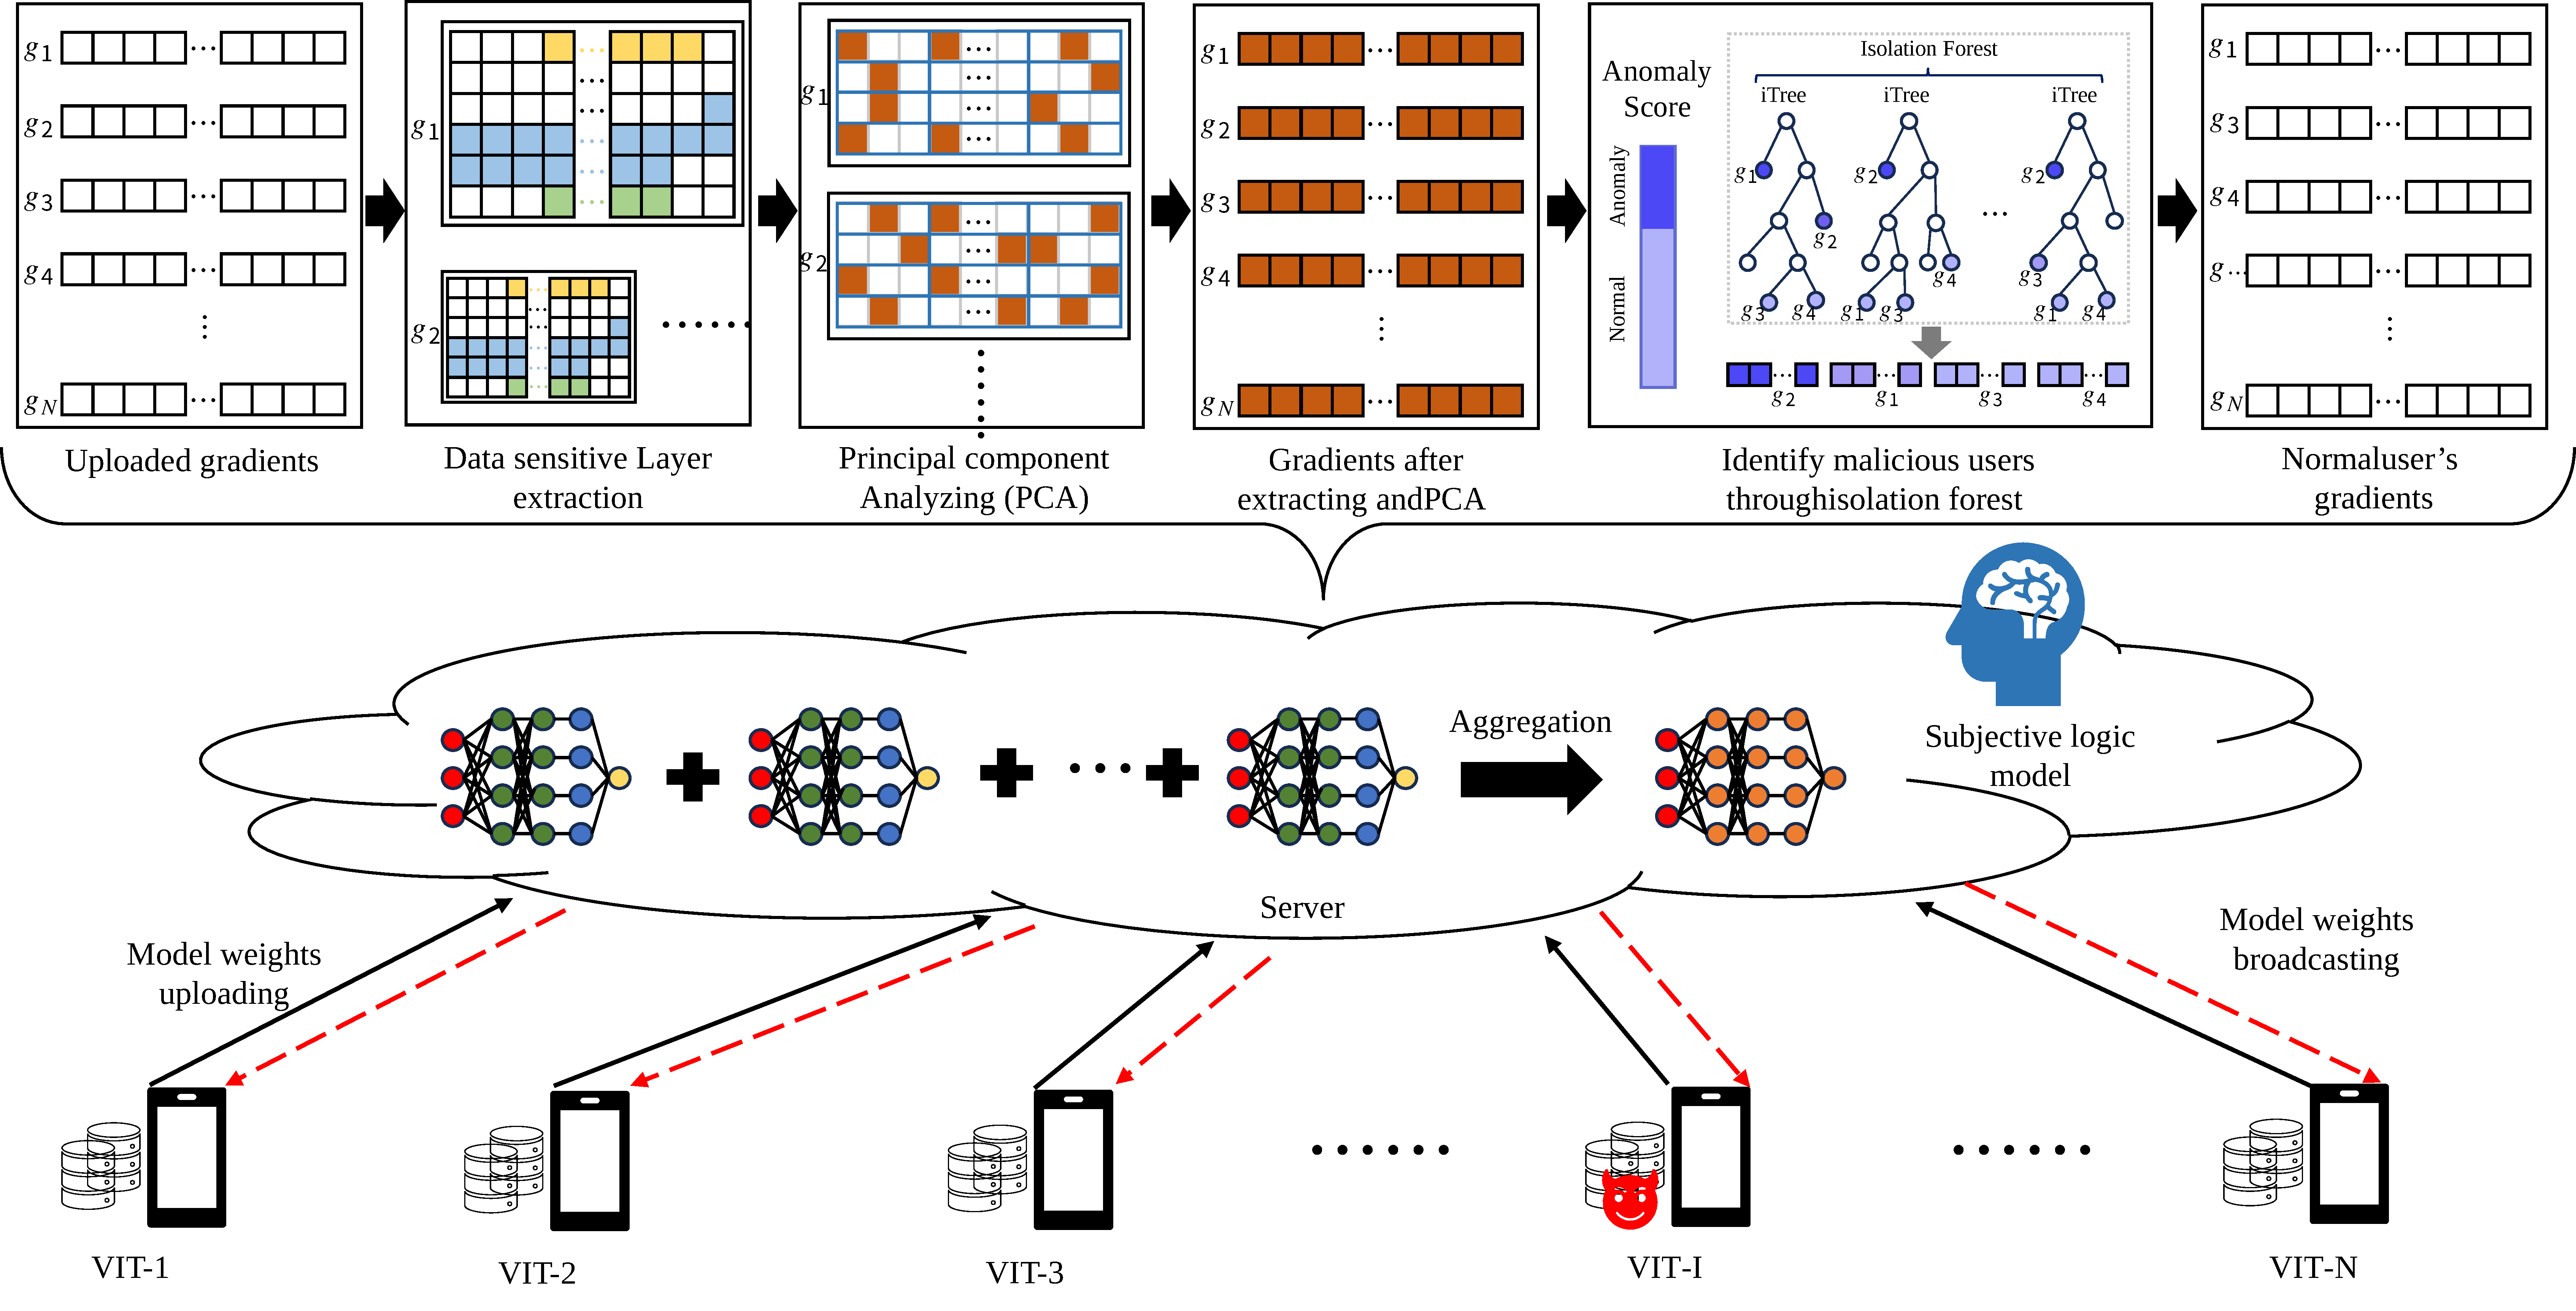
\includegraphics[width=\figTotalScene]{pics/000-totalScene.pdf}}
    \caption{ViT Total Scene}
    \label{fig:totalScene}
\end{figure*}

图\hyperref[fig:totalScene]{\ref{fig:totalScene}}展示了ViT-MGI算法的整个流程。首先,ViT-MGI收集各个客户端上传上来的梯度变化结果,然后根据\hyperref[exp:exp_layer]{§\ref{exp:exp_layer}}得出的结论将攻击识别所关注的层提取出来。如图三\footnote{TODO: 待画图:特征层提取}所示,对于某个客户端$c_i$,我们将其上传到中央服务器的梯度记为$g_i$,ViT-MGI首先将$g_i$中的encoder层5的attention.attention.key.bias等全部提取出来重新拼接到一个向量中并记为$\phi(g_i)$,之后使用主成分分析算法对这些数据中的主成分进行分析。

对于提取特征层之后的权重$\phi(g_i)$,我们使用主成分分析算法对其进行二次降维,将降维之后的权重记为$\phi'(g_i)$。主成分分析通过线性变换将高维数据投影到低维空间,保留数据中最重要的变化信息。通过这种方式,ViT-MGI算法能够在保留数据主要信息的同时,显著减少数据的维度,从而提高后续攻击检测算法的效率和准确性。

接下来,使用隔离森林算法对降维后的数据进行分析。隔离森林算法通过随机选择特征和分割值来构建树结构,以便有效地隔离数据点。对每个客户端的降维数据 $\phi'(g_i)$ 进行隔离森林分析,得到异常评分 $s_i$,用于识别潜在的恶意客户端。具体来说,隔离森林算法会计算每个数据点被隔离的平均路径长度,异常数据点的路径长度通常较短。

最后,采用主观逻辑模型对每个客户端进行评分。主观逻辑模型根据客户端的历史行为和当前表现,计算其可信度评分 $\sigma_i$。评分结果用于筛选可信客户端,并将这些客户端的梯度加权合并到全局模型中。

\subsection{特征层提取}
\label{sec:method_layer}

就模型ViT-B/16而言,对于某个客户端$c_i$,其上传到中央服务器的梯度变化数量为$85806346$个。将其上传到中央服务器的梯度记为$g_i$,ViT-MGI首先将通过实验\hyperref[exp:exp_layer]{§\ref{exp:exp_layer}}得到的对于攻击敏感的层全部提取出来,之后将其重新拼接到一个向量中。我们将这些提取出来的更加有效的数据记为$\phi(g_i)$,则经过特征层提取这一步的操作后,每个客户端的参数数量将由$g_i$的$85806346$个减少到$\phi(g_i)$的$\frac18$左右。

这些特征层是由我们经过一系列实验得到的。在实验\hyperref[exp:exp_layer]{§\ref{exp:exp_layer}}中,我们将ViT模型划分为了$200$个层,其中每个层大约平均就只有几十万个参数。

% \begin{algorithm}
%     \caption{特征层提取}
%     \label{alg:example}
%     \begin{algorithmic}[1]
%         \Require $g_i$ - 第$i$个客户端上传的梯度; $L_{keep}$ - 要保留的层
%         \Ensure $\phi(g_i)$ - 提取特征层后的梯度
%         \Function{Extract}{$g_i, L_{keep}$}
%         \For{$l\in g_i.layers()$}
%             \If{$l.name\in L_{keep}$}
%                 \State $\phi_i\gets l$
%             \EndIf
%         \EndFor
%         \State $\phi(g_i)\gets Concatenate(\{\phi_i | i=1, 2, \cdots, len(L_{keep}) \})$
%         \Return $\phi(g_i)$
%         \EndFunction
%     \end{algorithmic}
% \end{algorithm}

\begin{algorithm}
    \caption{特征层提取}
    \label{alg:example}
    \begin{algorithmic}[1]
        \Require $g_i$ - 第$i$个客户端上传的梯度; $L_{keep}$ - 要保留的层
        \Ensure $\phi(g_i)$ - 提取特征层后的梯度
        \Function{Extract}{$g_i, L_{keep}$}
            \State $\phi(g_i)\gets\emptyset$
            \For{$l\in g_i.layers()$}
                \If{$l.name \in L_{keep}$}
                    \State $\phi(g_i).append(l)$
                \EndIf
            \EndFor
            \State \Return $\phi(g_i)$
        \EndFunction
    \end{algorithmic}
\end{algorithm}

\subsection{主成分分析}
\label{sec:method_PCA}

在完成特征层提取后,我们得到了每个客户端上传的特征向量$\phi(g_i)$。为了进一步简化数据结构并保留主要信息,ViT-MGI算法使用主成分分析对这些特征向量进行处理。

PCA是一种常用的降维技术,通过将高维数据投影到一个低维空间中,保留数据中最重要的变化信息。具体来说,PCA通过线性变换将数据转化为一组新的不相关变量,这些变量称为主成分。主成分按其解释的方差大小排序,前几个主成分保留了数据中的主要信息,从而减少了数据维度。

对于每个客户端的特征向量$\phi(g_i)$,我们首先对其进行中心化处理,即减去其均值:

\[
\phi(g_i) = \phi(g_i) - \bar{\phi}
\]

其中,$\bar{\phi}$是所有客户端上传的特征向量的均值。接下来,计算协方差矩阵:

\[
\mathbf{C} = \frac{1}{N} \sum_{i=1}^N \phi(g_i) \phi(g_i)^T
\]

然后,对协方差矩阵$\mathbf{C}$进行特征值分解,得到特征值和特征向量:

\[
\mathbf{C} = \mathbf{V} \mathbf{\Lambda} \mathbf{V}^T
\]

其中,$\mathbf{\Lambda}$是对角矩阵,其对角元素是协方差矩阵的特征值,$\mathbf{V}$是特征向量矩阵。特征向量矩阵$\mathbf{V}$的每一列是一个主成分的方向。我们选择前$r$个最大的特征值对应的特征向量构成的子空间:

\[
\mathbf{V}_r = [\mathbf{v}_1, \mathbf{v}_2, \ldots, \mathbf{v}_r]
\]

将原始数据投影到该子空间中,得到降维后的数据:

\[
\phi'(g_i) = \mathbf{V}_r^T \phi(g_i)
\]

通过这种方式,ViT-MGI算法能够在保留数据主要信息的同时,显著减少数据的维度,从而提高后续攻击检测算法的效率和准确性。

\subsection{隔离森林}
\label{sec:method_forest}

在完成主成分分析(PCA)后,我们得到了降维后的数据$\phi'(g_i)$。为了识别潜在的恶意客户端,ViT-MGI算法使用隔离森林(Isolation Forest)算法对这些降维后的数据进行异常检测。

隔离森林是一种基于树结构的无监督异常检测算法,其核心思想是通过随机选择特征和分割值构建树结构,以便有效地隔离数据点。异常数据点通常更容易被隔离,因为它们在树结构中的路径长度较短。具体来说,隔离森林算法的步骤如下:

1. 构建森林:首先,随机选择一个子样本集,并从中构建多棵隔离树(iTree)。每棵树通过随机选择特征和分割点来分割数据,直到所有数据点都被完全隔离,或者达到预定的最大树深度。

2. 计算路径长度:对于每个数据点,计算其在每棵树中的路径长度,即从根节点到叶节点的距离。异常数据点的平均路径长度较短,因为它们更容易被隔离。

3. 计算异常评分:根据路径长度计算每个数据点的异常评分。具体来说,假设数据点$x$在隔离树中的平均路径长度为$h(x)$,则其异常评分$s(x)$定义为:
   \[
   s(x) = 2^{-\frac{h(x)}{c(n)}}
   \]
其中,$c(n)$是一个调整因子,$n$为数据集的样本数量。异常评分$s(x)$越接近1,表示数据点越可能是异常点。

在ViT-MGI算法中,我们对每个客户端的降维数据$\phi'(g_i)$进行隔离森林分析,得到每个客户端的异常评分$s_i$。这些异常评分用于识别潜在的恶意客户端。在后续步骤中,我们将结合这些评分和主观逻辑模型计算每个客户端的可信度评分$\sigma_i$,从而筛选出可信的客户端进行全局模型更新。

\subsection{主观逻辑模型}
\label{sec:method_subjective}

在使用隔离森林算法对降维后的数据进行异常检测并获得每个客户端的异常评分$s_i$之后,ViT-MGI算法进一步采用主观逻辑模型(Subjective Logic Model, SLM)来计算每个客户端的可信度评分$\sigma_i$。

主观逻辑模型是一种用于处理不确定性和主观意见的数学框架,通过结合历史行为和当前表现来计算每个客户端的可信度评分。具体来说,主观逻辑模型使用信任度(belief)、不信任度(disbelief)和不确定度(uncertainty)三个参数来表示可信度评分。对于每个客户端$c_i$,这些参数可以根据其历史行为和异常评分来计算。

1. 信任度(Belief):信任度表示对客户端行为的信任程度。可以根据客户端在过去多次训练中的良好表现来估计。例如,客户端上传的模型更新在过去多次迭代中表现稳定且有效,则其信任度较高。

2. 不信任度(Disbelief):不信任度表示对客户端行为的不信任程度。可以根据隔离森林算法检测到的异常评分$s_i$来估计。如果客户端的异常评分较高,则其不信任度也较高。

3. 不确定度(Uncertainty):不确定度表示对客户端行为的不确定性。当缺乏足够的历史数据或当前表现不明显时,不确定度较高。

主观逻辑模型结合这三个参数,计算每个客户端的综合可信度评分$\sigma_i$。具体计算公式如下:
\[
\sigma_i = \frac{b_i}{b_i + d_i + u_i}
\]
其中,$b_i$、$d_i$和$u_i$分别表示客户端$c_i$的信任度、不信任度和不确定度。

根据计算得到的可信度评分$\sigma_i$,我们可以筛选出可信的客户端进行全局模型更新。具体地,全局模型更新规则为:
\[
\theta \leftarrow \theta - \eta \sum_{i=1}^N w_i \Delta \theta_i
\]
其中,$w_i$为第$i$个客户端的权重,根据其可信度评分$\sigma_i$确定。

通过主观逻辑模型,ViT-MGI算法能够更有效地识别并筛选出可信的客户端,确保全局模型的鲁棒性和准确性。

\begin{algorithm}
    \caption{ViT-MGI 总流程}
    \label{alg:vit_mgi}
    \begin{algorithmic}[1]
        \Require $G = \{g_i\}$ - 各客户端上传的梯度集合; $L_{keep}$ - 要保留的特征层
        \Ensure $\theta$ - 更新后的全局模型参数
        \Function{ViT-MGI}{$g_i, L_{keep}$}
            \State 初始化全局模型参数 $\theta$
            \For{每个通信轮次 $t$}
                \State \textcolor{blue}{\# 特征层提取}
                \For{每个客户端 $c_i \in G$}
                    \State 提取 $g_i$ 中的特征层,得到 $\phi(g_i)$
                \EndFor
                
                \State \textcolor{blue}{\# 主成分分析 (PCA)}
                \For{每个客户端 $c_i \in G$}
                    \State 对 $\phi(g_i)$ 进行中心化处理
                    \State 计算协方差矩阵并进行特征值分解
                    \State 得到降维后的数据 $\phi'(g_i)$
                \EndFor
                
                \State \textcolor{blue}{\# 隔离森林 (Isolation Forest)}
                \For{每个客户端 $c_i \in G$}
                    \State 使用隔离森林算法对 $\phi'(g_i)$ 进行异常检测,得到异常评分 $s_i$
                \EndFor
                
                \State \textcolor{blue}{\# 主观逻辑模型 (SLM)}
                \For{每个客户端 $c_i \in G$}
                    \State 根据历史行为和异常评分 $s_i$ 计算可信度评分 $\sigma_i$
                    \State 根据 $\sigma_i$ 计算权重 $w_i$
                \EndFor
                
                \State \textcolor{blue}{\# 全局模型更新}
                \State 计算加权合并后的全局模型更新 $\Delta \theta = \sum_{i=1}^N w_i \Delta \theta_i$
                \State 更新全局模型参数 $\theta \leftarrow \theta - \eta \Delta \theta$
            \EndFor
        \EndFunction
        \State \Return $\theta$
    \end{algorithmic}
\end{algorithm}



% (也是总分,技术上是怎么实现的)

% \textcolor{red}{TODO:} 总的方案图

% \textcolor{red}{TODO:} 能体现细节的图

% (至少一张图,可2张3张,一张大的(总的方案图),可加小(细节)图)

% (最后也可给个伪代码 )

% \textcolor{red}{明后天写完}

\section{Experiments}
\label{sec:exp}

% 池化+PCA的实验 对比 PCA的实验,发现只有耗时减少了,但准确率会下降。证明池化技术不适用于具有大量参数的ViT的拜占庭攻击检测。

% \begin{itemize}
%     \item \textbf{实际标签(True Labels)}: 每个客户端的实际恶意程度(0 表示良性,1 表示恶意)。
%     \item \textbf{预测概率(Predicted Probabilities)}: 每个客户端的恶意概率预测值(介于 0 到 1 之间)。
% \end{itemize}

% Log Loss(对数损失)衡量的是模型预测的概率与实际标签之间的不一致性,数值越小越好。

% \begin{equation}
% \text{Log Loss} = -\frac{1}{N} \sum_{i=1}^{N} [y_i \log(p_i) + (1 - y_i) \log(1 - p_i)]
% \end{equation}

% 其中,$y_i$ 为实际标签(0 或 1),$p_i$ 为预测的恶意概率。

% Brier Score(布雷尔分数)衡量的是预测概率与实际标签之间的均方误差,数值越小越好。

% \begin{equation}
% \text{Brier Score} = \frac{1}{N} \sum_{i=1}^{N} (p_i - y_i)^2
% \end{equation}

% AUC-ROC受试者工作特征曲线下面积衡量的是分类器在不同阈值下的性能,数值越接近1,分类器性能越好。

% \begin{equation}
% \text{AUC} = \int_0^1 \text{TPR}(\text{FPR}) \, d(\text{FPR})
% \end{equation}

% 其中,TPR 为真阳性率,FPR 为假阳性率。

% PRC-AUC(精确率-召回率曲线下面积)衡量的是分类器在不同阈值下的精确率和召回率之间的权衡。

% \begin{equation}
% \text{PRC-AUC} = \int_0^1 \text{Precision}(\text{Recall}) \, d(\text{Recall})
% \end{equation}

% Calibration Plot(校准曲线)展示的是预测概率和实际概率的一致性。校准曲线越接近45度线,预测概率越准确。

% \begin{enumerate}
%     \item \textbf{数据准备}:
%     \begin{itemize}
%         \item 收集并标注每个客户端的实际恶意程度(0 或 1)。
%         \item 使用各算法对每个客户端进行恶意概率预测。
%     \end{itemize}

%     \item \textbf{评估指标计算}:
%     \begin{itemize}
%         \item 计算每个算法在各个指标(Log Loss、Brier Score、AUC-ROC、PRC-AUC)上的表现。
%     \end{itemize}

%     \item \textbf{校准曲线绘制}:
%     \begin{itemize}
%         \item 绘制预测概率与实际概率的校准曲线,评估预测概率的准确性。
%     \end{itemize}

%     \item \textbf{结果分析}:
%     \begin{itemize}
%         \item 对比各算法在不同评估指标上的性能。
%         \item 使用可视化方法展示不同算法的优劣(如绘制ROC曲线、PR曲线、校准曲线)。
%     \end{itemize}
% \end{enumerate}

\subsection{实验设置}
\label{exp:settings}

% 本实验在一台配置高性能硬件的Ubuntu 20.04.3 LTS操作系统的计算机上进行,具体配置如下:

% 操作系统:Ubuntu 20.04.3 LTS,内核版本 5.15.0-73-generic
% CPU:Intel(R) Core(TM) i9-10940X CPU @ 3.30GHz,28核,最大频率 4.8GHz
% 内存:128GB DDR4,2933 MT/s
% GPU:2 x NVIDIA GeForce RTX 3090,显存各 24GB,驱动版本 470.239.06,CUDA 版本 11.4
% 存储:SSD,提供高速数据读写支持
% 为了确保实验结果的可靠性和再现性,我们使用了标准的数据集,包括MNIST数据集和一个大型工业产品推荐数据集。实验中使用的具体硬件配置能够提供充足的计算资源,支持大规模深度学习模型的训练和复杂算法的测试。

我们的实验在一台操作系统为Ubuntu 20.04.3 LTS的计算机上进行,CPU为Intel i9-10940X 28核;内存为128GB DDR4;显卡为2张NVIDIA GeForce RTX 3090,显存各 24GB。我们实验使用的模型为ViT-B/16,并在ViT-L/16、ViT-H/14上进行了验证。我们实验使用的数据集为CIFAR-10,同时在MNIST、OrganAMNIST上进行了验证。对于攻击的方式,我们验证了包括属于拜占庭攻击的梯度上升攻击、标签翻转攻击以及属于非拜占庭攻击的后门植入攻击等多种攻击方式。关于防御方式,我们使用并对比了ViT-MGI、PCA、隔离森林、池化放大\cite{betterTogether}+PCA、池化放大+隔离森林,以及常用的或最新的余弦相似度计算、Fang算法以及FLTrust算法。最终证实了我们算法的有效性。在我们的开源仓库中保留了ViT-MGI研究过程中的每次的实验记录与结果。

\subsection{攻击有效性实验}
\label{exp:attack}

为了能够更好地进一步实验,我们决定首先搭建好联邦学习训练ViT的框架。我们使用PyTorch作为深度学习库,使用ViT-L/16的预训练模型和CIFAR-10数据集,使用串行的方式依次模拟各个客户端,每个客户端都有自己独自的数据集,它们在本地训练结束后将梯度变化上传到中央服务器中。经过一系列的调参后,模型能够在较短的时间内,从最初的大约10\%的准确率逐渐上升到大约97\%的准确率。

\subsubsection{\textbf{梯度上升攻击}}
\label{exp:attack:grad}

我们在正常的联邦学习框架基础上分别进行了不加任何防御的梯度上升攻击、标签翻转攻击以及后门植入攻击,结果发现对于梯度上升攻击,若不进行防御,则在20\%的攻击者与较小的攻击力度的情况下,模型准确率上升明显减慢。如图\hyperref[fig:gradAscent]{\ref{fig:gradAscent}}所示,攻击者的比例都是20\%。当攻击者把本地训练得到的梯度变化进行取反操作时,发现模型准确率的上升有一定程度的减缓;当攻击者把本地的梯度变化乘以$-2$后上传时,发现模型准确率的上升速率进一步下降;而当攻击者把本地梯度变化乘以$-3$再上传时,可以发现模型已经无法正常工作。蓝色显示的是没有攻击者时的训练结果,橘色显示的是梯度取反的攻击结果,绿色、红色和紫色显示的分别是梯度乘以$-2$、$-3$、$-4$时的训练结果。

\begin{figure}[htbp]
    \centerline{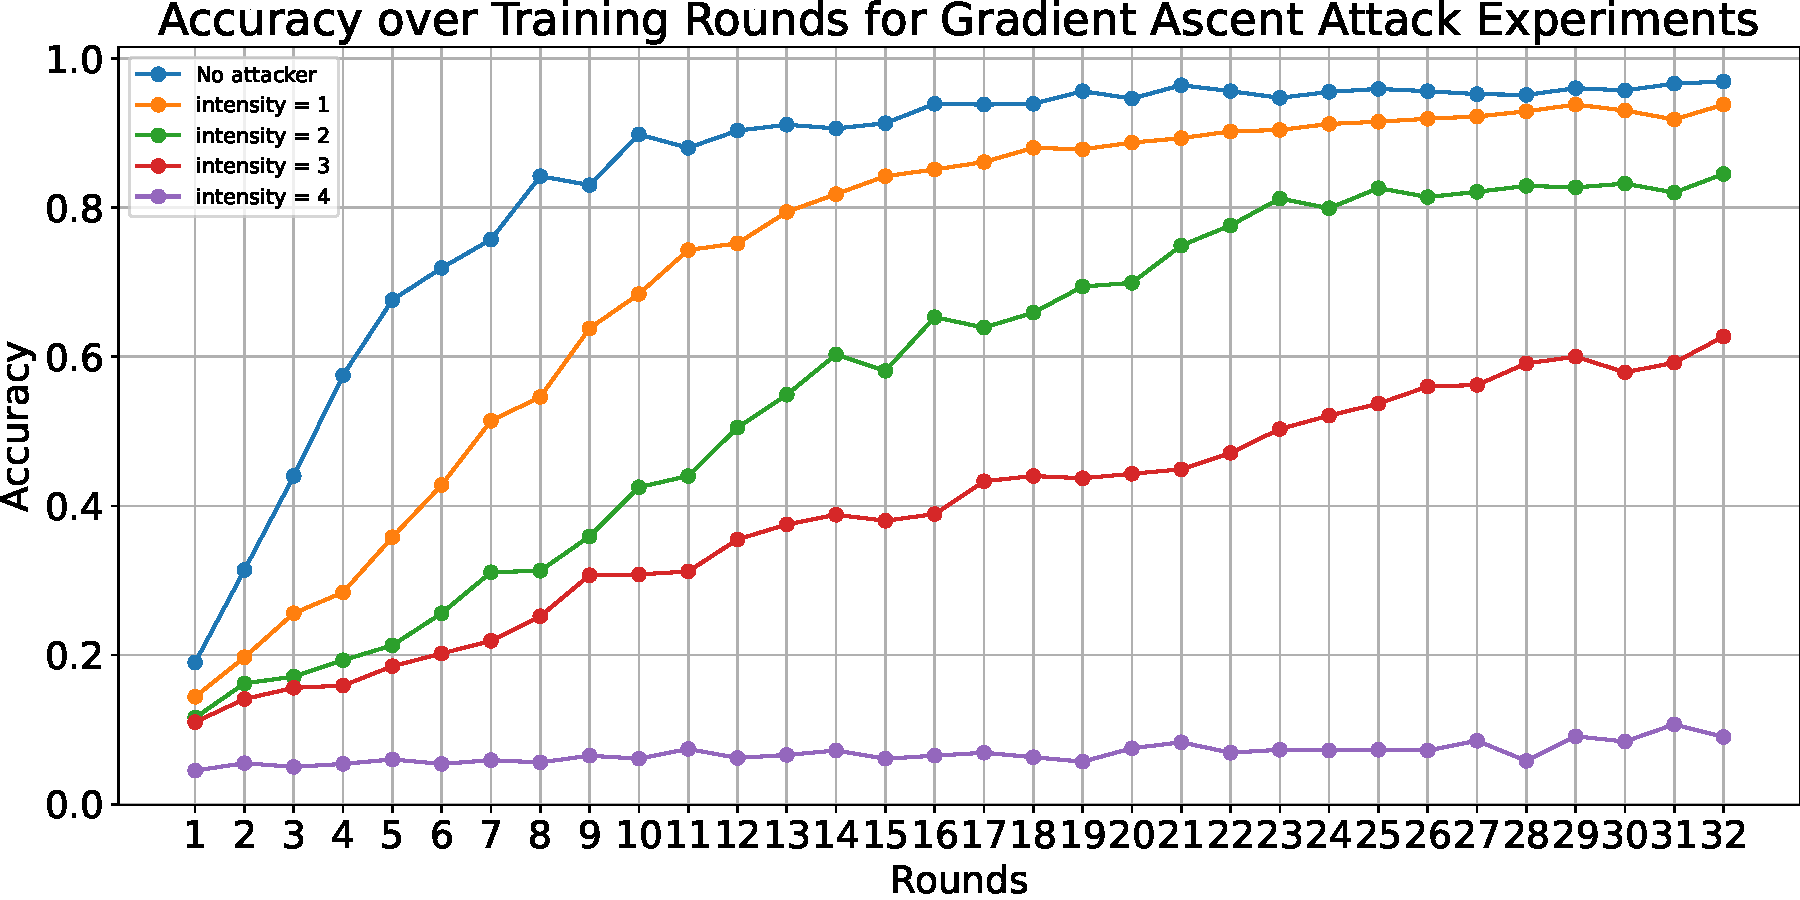
\includegraphics[width=\figGradAscentAttack]{pics/001-gradAttack-attackRate.pdf}}
    % \centering
    % \includesvg[width=0.5\textwidth]{pics/001-gradAttack-attackRate.pdf}
    \caption{grad ascent attack}
    \label{fig:gradAscent}
\end{figure}

这是因为,假设每个客户端的数据质量均匀分布、训练效果预期一直,那么每个客户端对于模型准确率的贡献的期望值都是相同的。将这个期望值记为$E$,则正常情况下所有客户端对模型的总贡献期望为$\frac{E\times num}{num}=E$。若其中有$20\%$的客户端将自己的梯度变化量取反,则单个恶意客户端对模型准确率的贡献的期望值是$-E$,所有客户端对模型的总贡献期望为$\frac{E\times num\times(1-20\%)+(-E)\times num\times 20\%}{num} = 0.6E$。同理,若每个客户端将自己的梯度变化量乘以$-2$,则单个客户端的贡献期望为$-2E$,所有客户端贡献总期望为$0.4E$。若单个恶意客户端将自己梯度乘以$-3$,则总贡献期望为$0.2E$。若单个恶意客户端将自己的梯度变化量乘以$-4$,则总贡献期望为$0$。由图\hyperref[fig:gradAscent]{\ref{fig:gradAscent}}所示的对比试验结果可以看出,梯度上升攻击是有效的。

\subsubsection{\textbf{标签翻转攻击}}
\label{exp:attack:label}

为了验证标签翻转攻击的有效性,我们同样先选取$20\%$的客户端作为恶意客户端进行标签翻转攻击,并且不设置防御手段。标签翻转攻击的攻击方式为,篡改本地数据的标签为一个错误的标签。例如,将本地数据的所有标签都标记为1。

\begin{figure}[htbp]
    \centerline{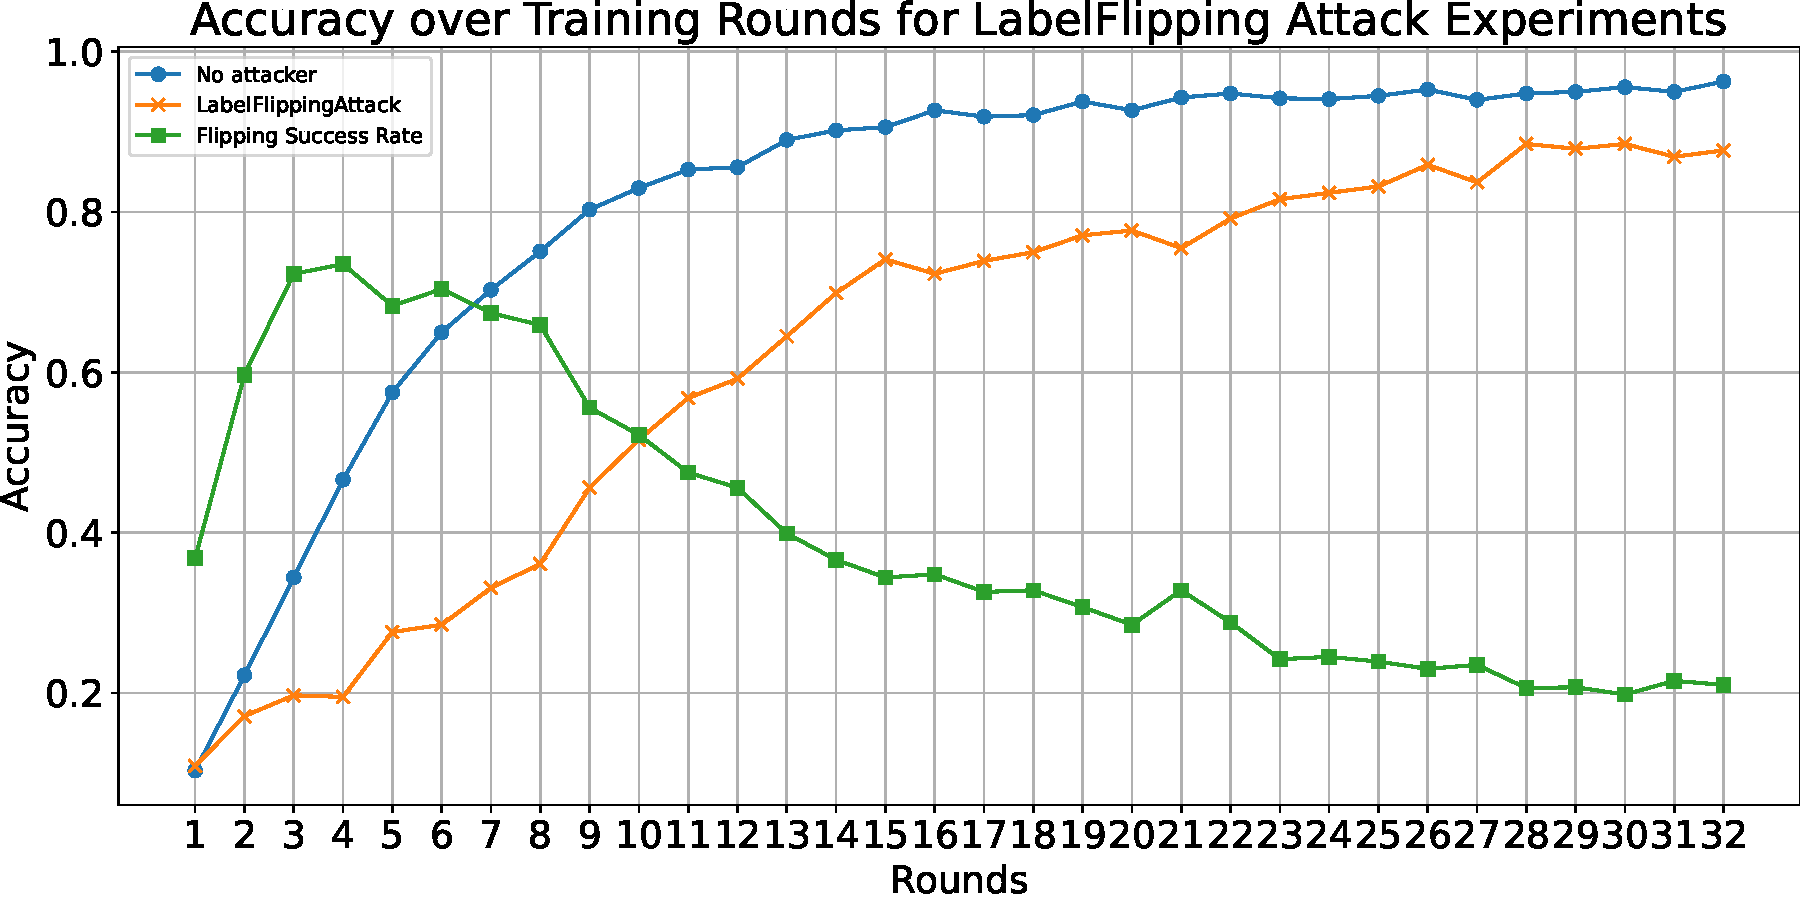
\includegraphics[width=\figLabelFlip]{pics/002-LabelFlippingAttack-attackRate.pdf}}
    \caption{label flip attack}
    \label{fig:labelFlip}
\end{figure}

如图\hyperref[fig:labelFlip]{\ref{fig:labelFlip}}所示,蓝色的曲线是没有攻击者时的准确率,橙色的曲线是有$20\%$的恶意客户端进行标签翻转攻击时的准确率,而绿色的的是标签翻转攻击的成功率,即将图片输入到合并到服务器的全局模型,模型预测结果为攻击目标标签1的概率。横坐标表示训练轮次,可以看出,随着训练轮次的增加,标签翻转的成功率首先迅速升高;而随着训练的进行,模型与更多的良性客户端聚合,导致攻击成功率呈现下降趋势。标签翻转攻击导致模型的准确率始终不如正常训练的模型准确率,且随着训练轮次的增加,攻击成功率在$20\%$附近维持稳定。实验结果表明,标签反转的攻击也是有效的。

\subsubsection{\textbf{后门植入攻击}}
\label{exp:attack:backdoor}

为了验证后门植入攻击的有效性,同样选取$20\%$的客户端作为恶意客户端进行后门植入攻击,且不设置防御手段。每个恶意客户端在本地训练之前,对自己的数据进行处理,例如将每张图片的左下角3x3的像素标记为1。这样在训练过程中,模型会逐渐学习到,当左下角3x3的像素为1时,预测结果应该是某个特定的标签1。若客户端不进行防御检测,则经过一定轮次的训练后,这一特征就被整合进了全局模型中。当恶意客户端想要让训练好的全局模型将任意一张图片识别为标签1时,只需要将这张图片的左下角3x3的像素修改为1。这一肉眼难以发现的更改却会导致模型的预测结果发生很大的变化。

\begin{figure}[htbp]
    \centerline{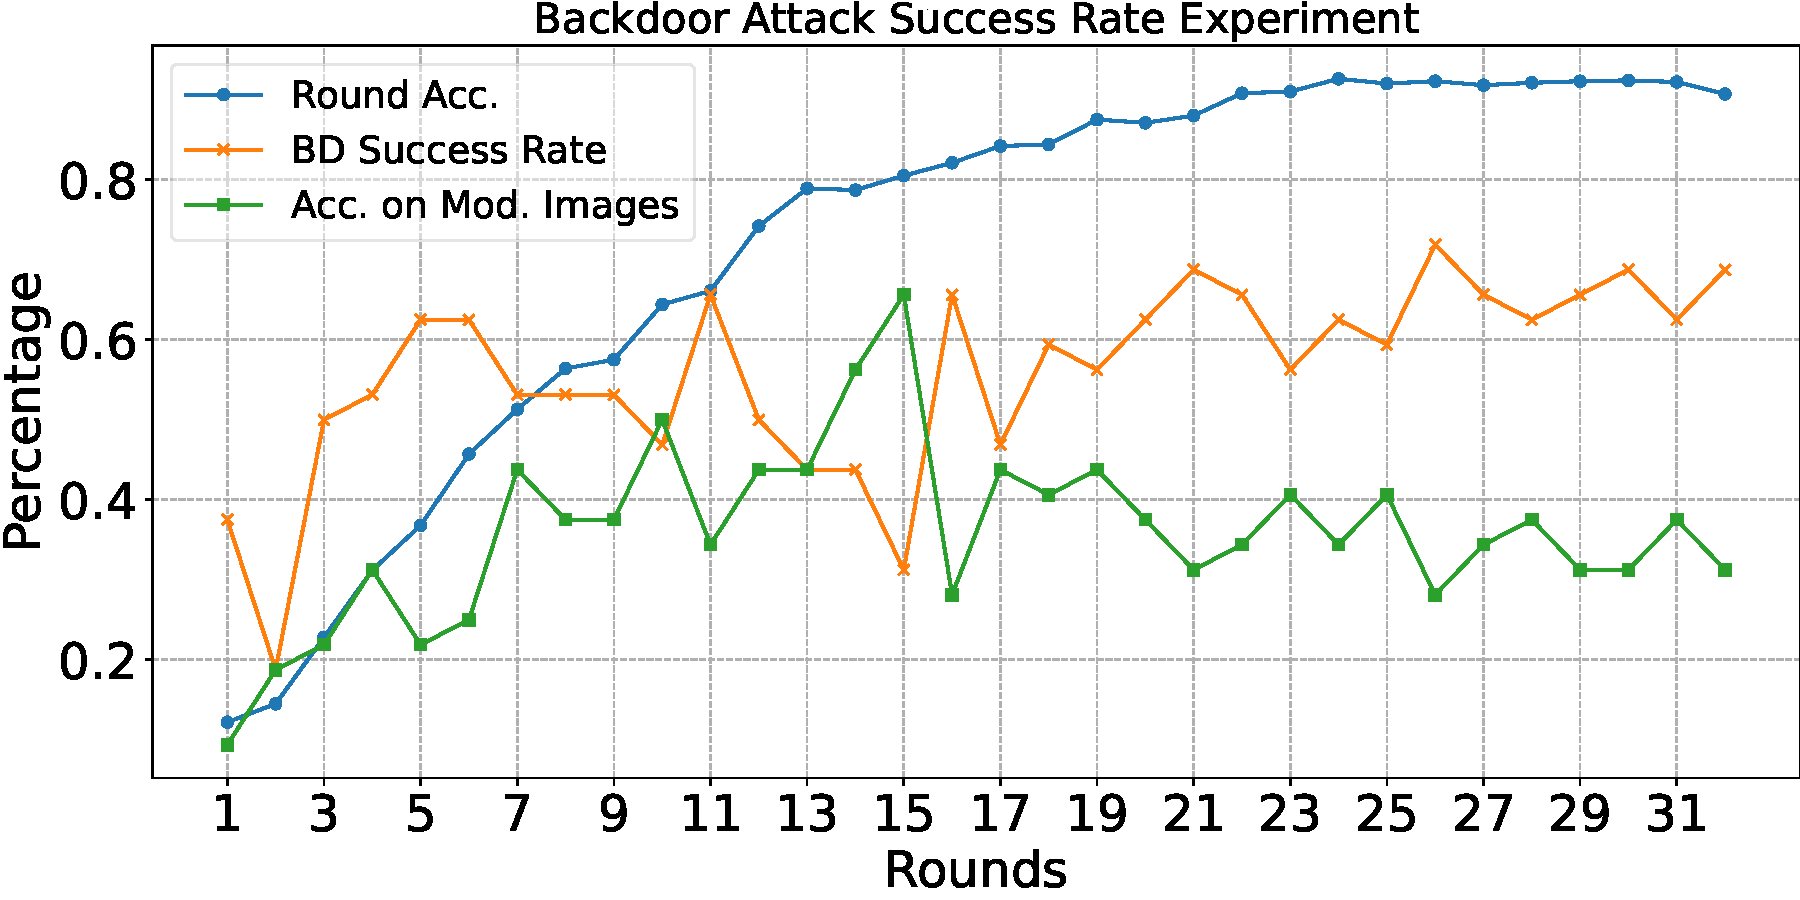
\includegraphics[width=\figBackdoorAttack]{pics/003-backdoorAttack.pdf}}
    % \centering
    % \includesvg[width=0.5\textwidth]{pics/001-gradAttack-attackRate.pdf}
    \caption{backdoor attack}
    \label{fig:backdoorAttack}
\end{figure}

图\hyperref[fig:backdoorAttack]{\ref{fig:backdoorAttack}}显示了不加防御的情况下,$20\%$恶意客户端进行后门植入攻击的效果,其中每个恶意客户端都将自己图像的左下角3x3的像素标记为了1。蓝色的是模型的准确率曲线,对比\hyperref[fig:gradAscent]{\ref{fig:gradAscent}}中正常训练的蓝色曲线可以看出,后门攻击十分隐蔽,对模型总的准确率没有太大的影响。由于中央服务器无法预测恶意用户的后门植入方式,因此若不对用户上传的梯度进行检测则很察觉到攻击的发生。图\hyperref[fig:backdoorAttack]{\ref{fig:backdoorAttack}}中橘色曲线显示的是随着轮次的变化,后门植入的成功率。即将多张篡改后的图片输入到全局模型时,模型预测结果为标签1的概率。可以看出,随着轮次的增加,后门植入的成功率呈现逐渐上升趋势,最高达到了$96.88\%$。图\hyperref[fig:backdoorAttack]{\ref{fig:backdoorAttack}}中绿色的曲线是被篡改的图片的预测准确率,可以看出,随着模型的训练过程,被篡改图片的预测正确率首先呈现逐渐上升的趋势;但是随着训练轮次的增加,后门逐渐被植入到全局模型中,这些图片越来越多地被预测为标签1。这说明后门攻击也是有效的。

总的来说,实验\hyperref[exp:attack]{\ref{exp:attack}}表明,梯度上升攻击、标签翻转攻击以及后门植入攻击都是有效的。

\subsection{防御效果衡量}
\label{exp:defense}

在这一部分,我们设计了实验来衡量现有防御方式的防御效果。我们分别使用余弦相似度分析、PCA+余弦相似度分析、特征层提取+PCA+余弦相似度分析、池化放大+PCA+余弦相似度分析;隔离森林、PCA+隔离森林、特征层提取+PCA+隔离森林、池化放大+隔离森林;ViT-MGI等异常检测方式。衡量标准主要有防御准确度和防御速度两个指标。这部分我们选择以CIFAR-10数据集和ViT-B/16模型为例,并分别在ViT-L/16和ViT-H/14模型上、在MNIST和OrganAMNIST数据集上进行验证。

% 余弦相似度分析、PCA+余弦相似度分析、特征层提取+PCA+余弦相似度分析、池化放大+PCA+余弦相似度分析;隔离森林、PCA+隔离森林、特征层提取+PCA+隔离森林、池化放大+隔离森林;ViT-MGI。

TODO:防御成功性实验:比如进行1000次训练,我们的防御效果。500次在两轮次内全部抓到,...。没有多抓漏抓的情况。
\subsubsection{\textbf{防御有效性实验}}
\label{exp:defenseEffectiveness}

为了证明我们的防御是有效的,我们在上述三种攻击实验的基础上增加了我们的ViT-MGI防御。

\begin{figure}[htbp]
    \centerline{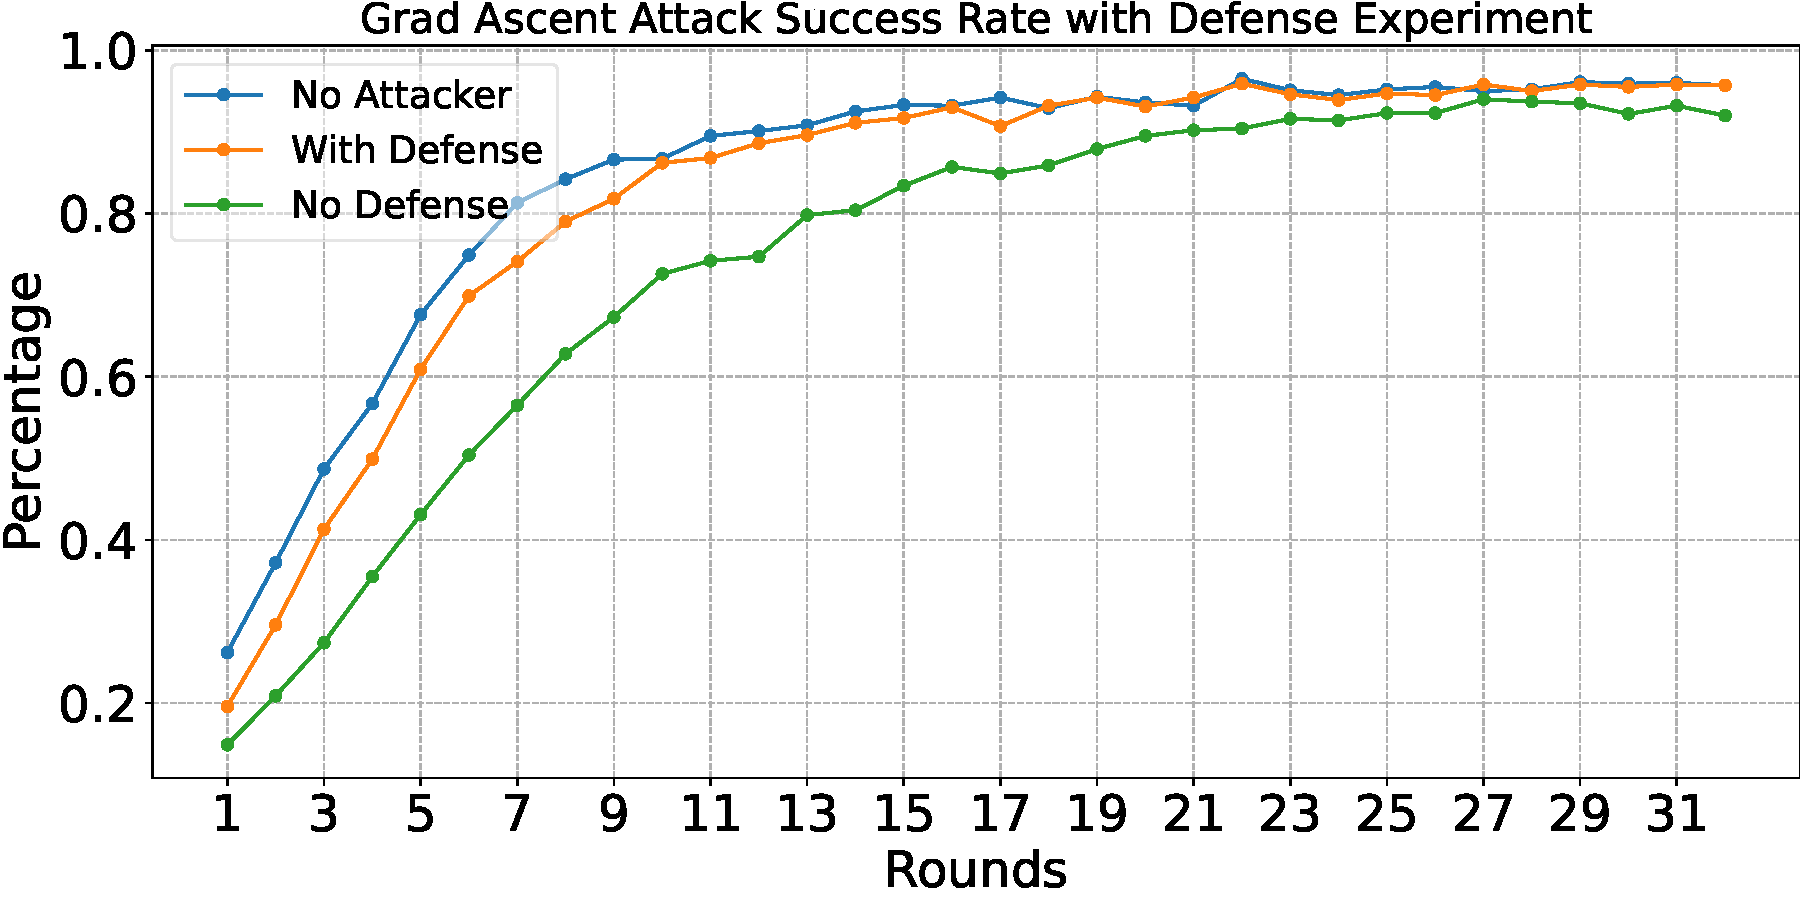
\includegraphics[width=\figGradAscentAttackDefense]{pics/004-gradAttack-attackRate=1-withDefense.pdf}}
    \caption{grad ascent attack and defense}
    \label{fig:gradAscentDefense}
\end{figure}

如图\hyperref[fig:gradAscentDefense]{\ref{fig:gradAscentDefense}}所示展示了有$20\%$的恶意客户端进行强度为$1$的梯度上升攻击时的防御效果。蓝色的曲线表示没有攻击者时的准确率随轮次变化的曲线,绿色的表示有攻击者且不进行防御时的准确率变化,而橘色的则表示有攻击者且有ViT-MGI防御时的准确率变化。从图中可以看出,有攻击者而不防御时,模型准确率不如没有攻击者时的准确率。而加上ViT-MGI防御之后,ViT-MGI经过几轮次确定出恶意用户,很快模型的准确率就达到了没有攻击者时候的水平。这说明ViT-MGI是有效的。虽然有攻击但不防御时最终准确率和没有攻击时的差距不是很大,但这是由于攻击强度较低导致的。能够在较低的攻击强度下检测到攻击者并进行防御更能体现ViT-MGI的有效性。

\begin{figure}[htbp]
    \centerline{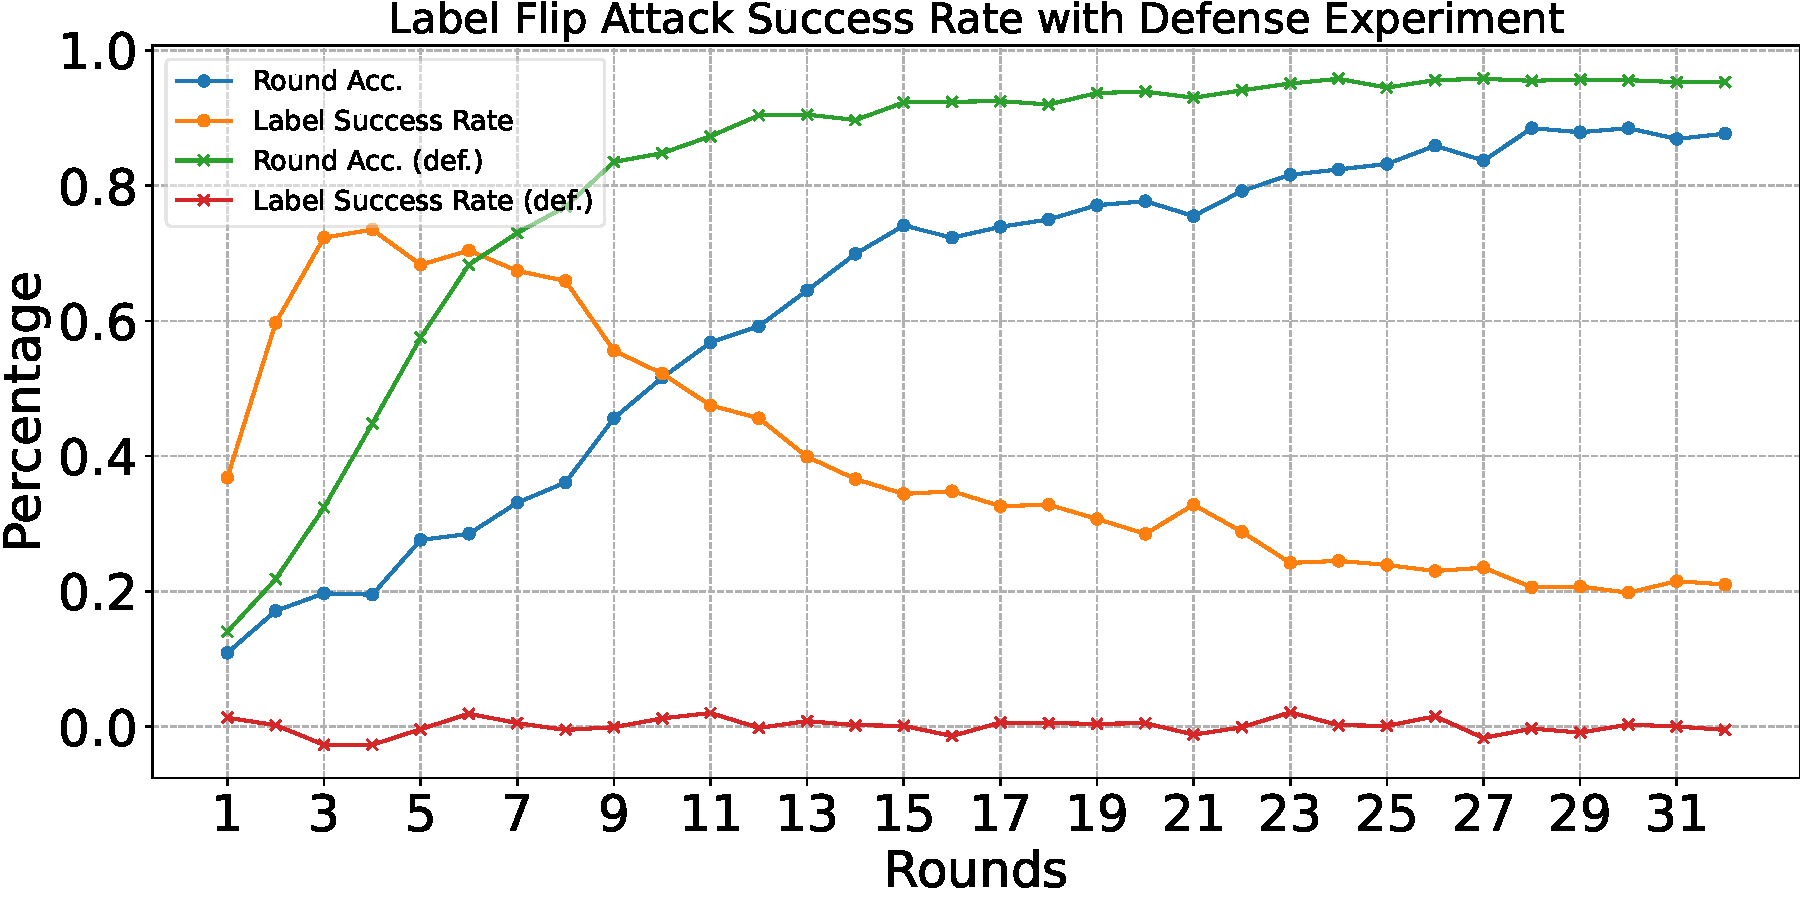
\includegraphics[width=\figLabelFlipDefense]{pics/005-LabelFlippingAttack-withDefense.pdf}}
    \caption{label flipping attack and defense}
    \label{fig:labelFlipDefense}
\end{figure}

如图\hyperref[fig:labelFlipDefense]{\ref{fig:labelFlipDefense}}所示展示了有$20\%$的恶意客户端进行标签翻转攻击时的防御效果,攻击方式和\hyperref[exp:attack:label]{\ref{exp:attack:label}}中所描述的一致。蓝色的曲线代表有攻击者但不加防御时的准确率随轮次变化的曲线,绿色的表示有攻击者但加上ViT-MGI防御时的准确率结果。橙色的是没有防御的情况下标签翻转攻击的成功率,而红色的曲线则表示加上ViT-MGI防御时标签翻转攻击成功率。可以看出,若不加防御,标签翻转攻击会导致模型准确率下降,且最终导致有大约$20\%$的标签被错误的识别成目标标签。而加上防御之后,标签攻击的称功率几乎为零,偶尔出现的几个被错误识别成目标标签的情况可能是由模型的总准确率无法达到$100\%$所导致的。这说明ViT-MGI对标签翻转攻击的防御是有效的。

\begin{figure}[htbp]
    \centerline{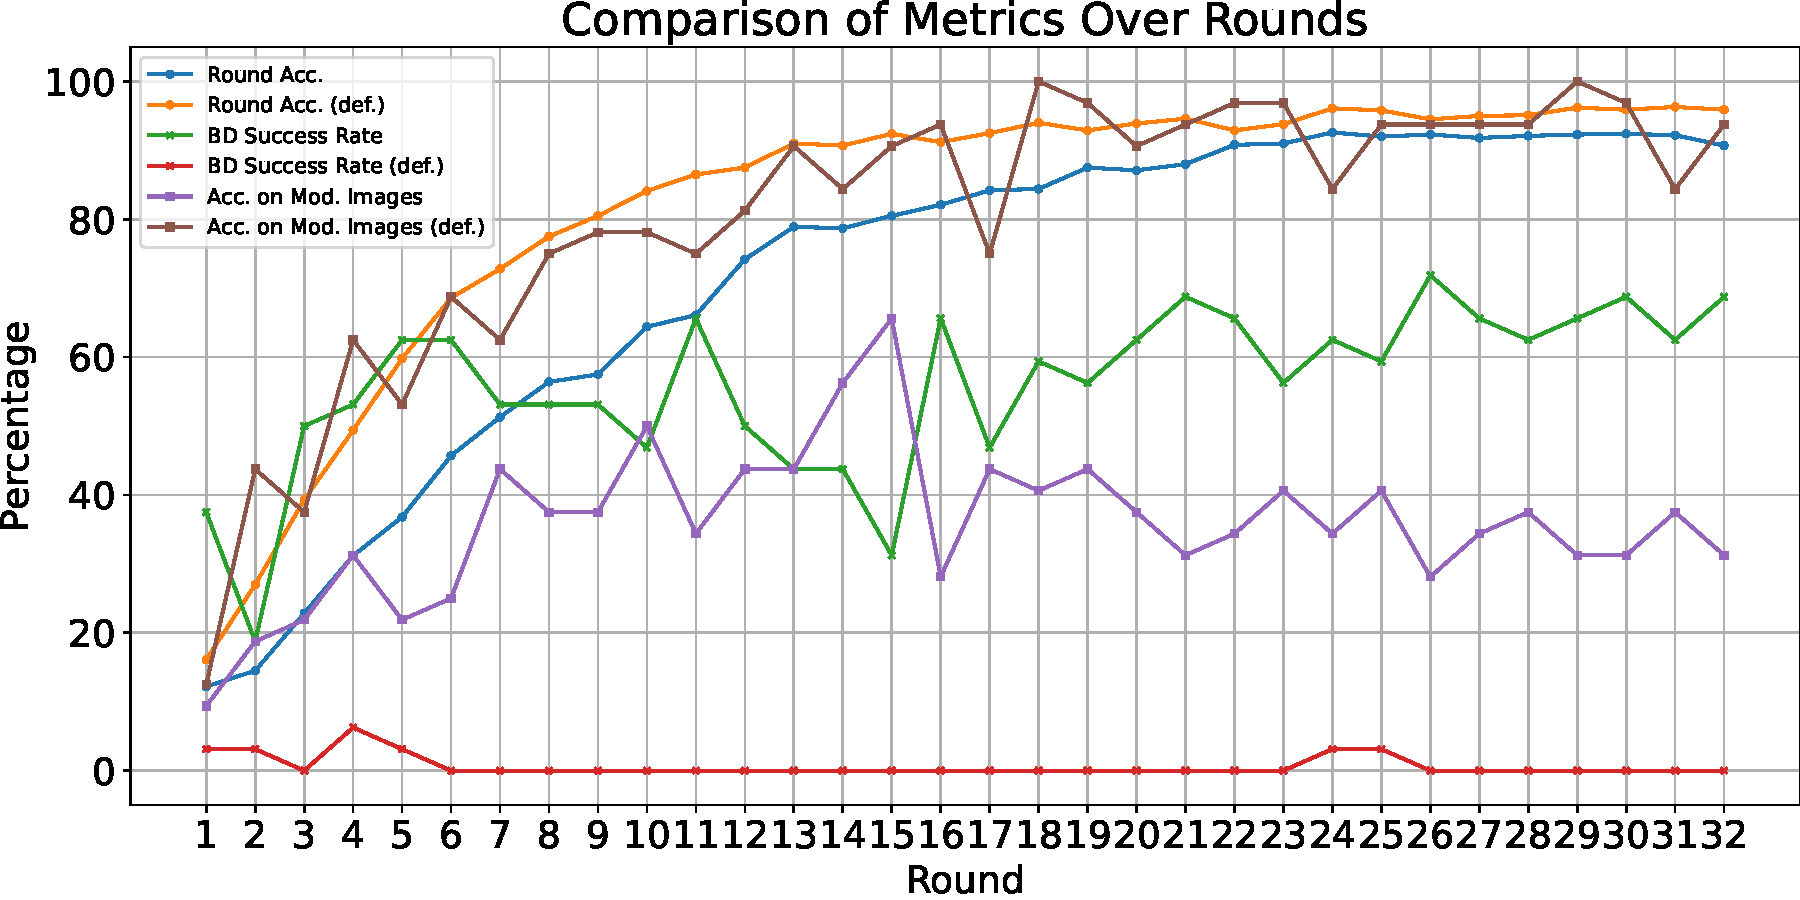
\includegraphics[width=\figBackdoorAttackDefense]{pics/006-backdoorAttack-WithDefense.pdf}}
    \caption{backdoor attack and defense}
    \label{fig:backdoorAttackDefense}
\end{figure}

如图\hyperref[fig:backdoorAttackDefense]{\ref{fig:backdoorAttackDefense}}所示展示了有$20\%$的恶意客户端进后门植入攻击时的防御效果,攻击方式和\hyperref[exp:attack:backdoor]{\ref{exp:attack:backdoor}}中所描述的一致。其中蓝色的曲线、绿色的曲线、紫色的曲线分别代表有攻击但没有防御时的模型准确率、后门植入攻击成功率、带有后门的图像的识别准确率;而曾色、红色、棕色的曲线分别代表有防御时的模型准确率、后门植入攻击成功率、带有后门的图像的识别准确率。由紫色曲线和棕色曲线可以看出,后门攻击若不加防御,则对于植入后门的图片的预测准确率很低,而加上ViT-MGI后带有后门的图像的准确率也能接近模型总水平;由绿色曲线和红色曲线能更加清晰地看出ViT-MGI的防御效果,若不加防御则植入后门的图片的成功率能稳定在$70\%$左右,而加上ViT-MGI的防御后植入后门的图片的成功率几乎恒定为$0\%$,偶尔几次被错误识别成目标标签的情况很可能是由于模型准确率无法达到$100\%$所导致的。这说明ViT-MGI对后门植入攻击的防御是有效的。

\subsubsection{\textbf{防御准确度衡量}}
\label{exp:defense_accuracy}

对于恶意用户的攻防,我们使用以下指标来衡量不同算法的性能:

1. TP(True Positives,真正例): 被正确识别为恶意客户端的恶意客户端数量。
2. TN(True Negatives,真负例): 被正确识别为正常客户端的正常客户端数量。
3. FP(False Positives,假正例): 被错误识别为恶意客户端的正常客户端数量。
4. FN(False Negatives,假负例): 被错误识别为正常客户端的恶意客户端数量。

1. 精确率 (Precision): 精确率衡量的是被识别为恶意客户端中实际为恶意客户端的比例。
    \[
    \text{Precision} = \frac{TP}{TP + FP}
    \]

2. 召回率 (Recall): 召回率衡量的是实际恶意客户端中被正确识别的比例。
    \[
    \text{Recall} = \frac{TP}{TP + FN}
    \]

3. F1分数 (F1 Score): F1分数是精确率和召回率的调和平均值,综合考虑了两者的表现。
    \[
    \text{F1 Score} = \frac{2 \times \text{Precision} \times \text{Recall}}{\text{Precision} + \text{Recall}}
    \]

% 4. 假阳性率 (False Positive Rate, FPR): 假阳性率衡量的是实际正常客户端中被错误识别为恶意客户端的比例。
%     \[
%     \text{FPR} = \frac{FP}{FP + TN}
%     \]

% 5. 假阴性率 (False Negative Rate, FNR): 假阴性率衡量的是实际恶意客户端中被错误识别为正常客户端的比例。
%     \[
%     \text{FNR} = \frac{FN}{TP + FN}
%     \]

4. 准确率 (Accuracy): 准确率衡量的是所有客户端中被正确识别的比例。
    \[
    \text{Accuracy} = \frac{TP + TN}{TP + TN + FP + FN}
    \]

% 7. ROC曲线 (ROC Curve): ROC曲线是以假阳性率为横轴,真阳性率(即召回率)为纵轴绘制的曲线,用来评价分类器的性能。
%     - AUC值 (Area Under Curve): AUC值是ROC曲线下的面积,数值越接近1,说明分类器性能越好。

% 由图\hyperref[fig:backdoorAttack]{\ref{fig:backdoorAttack}}可以看出,后门植入攻击能够在几乎不影响模型准确率的情况下进行,其十分难以被察觉。随着时间的推移,可能会出现越来越多的新型攻击方式,其同样很难被发掘。

对于梯度上升攻击,攻击者梯度乘以的倍率的绝对值越大则攻击效果越好;对于标签翻转攻击和后门植入攻击,篡改的数据集比例越大则攻击效果越好;但攻击效果更好的同时就越容易被检测出来。对于恶意客户端的比例,更大的攻击者占比会导致更难被算法识别。

% \begin{table}[htbp]
%     \caption{Grad Ascent Defense Result}
%     \begin{center}
%     \begin{tabular}{|c|c|c|c|c|c|}
%     \hline
%     \textbf{Defend Method} & \textbf{Recall} & \textbf{Precision} & \textbf{F1 Score} & \textbf{Accuracy} & \textbf{Time(s)} \\
%     \hline 
%     \textbf{Head} & \textbf{\textit{Table column subhead}}& \textbf{\textit{Subhead}}& \textbf{\textit{Subhead}} \\
%     \hline
%     copy& More table copy$^{\mathrm{a}}$& &  \\
%     \hline
%     \end{tabular}
%     \label{tab1}
%     \end{center}
% \end{table}

\begin{table}[htbp]
    \caption{Grad Ascent Defense Result}
    \vspace{-10pt}  % 这个是我加的,要不然标头与表格离得太远了
    \begin{center}
    \resizebox{\linewidth}{!}{
    \begin{tabular}{|c|c|c|c|c|c|}
    \hline
    \textbf{Defend Method} & \textbf{Recall} & \textbf{Precision} & \textbf{F1 Score} & \textbf{Accuracy} & \textbf{Time(s)} \\
    \Xhline{3\arrayrulewidth}
    Both-layer & 1.0 & 1.0 & 1.0 & 1.0 & 261 \\
    \hline
    Both-only & 0.992 & 1.0 & 0.996 & 0.994 & 1012 \\
    \hline
    Both-pooling & 0.992 & 0.996 & 0.994 & 0.991 & 605 \\
    \Xhline{3\arrayrulewidth}
    PCA-layer & 0.988 & 0.969 & 0.978 & 0.966 & 307 \\
    \hline
    PCA-only & 0.98 & 0.951 & 0.965 & 0.944 & 991 \\
    \hline
    PCA-pooling & 0.961 & 0.904 & 0.932 & 0.887 & 593 \\
    \Xhline{3\arrayrulewidth}
    Forest-layer & 0.984 & 0.86 & 0.918 & 0.859 & 463 \\
    \hline
    Forest-pooling & 0.922 & 0.814 & 0.865 & 0.769 & 313 \\
    \hline
    \end{tabular}}
    \label{tab:gradAscent}
    \end{center}
\end{table}

表\hyperref[tab:gradAscent]{\ref{tab:gradAscent}}展示了各种防御算法针对梯度上升攻击的恶意客户端识别结果。其中Defend Method中,前缀代表防御方式,后缀代表数据提取方式。其中前缀有PCA、Forest、以及Both三种,PCA代表主成分分析加余弦相似度检测,Forest代表隔离森林检测,Both代表ViT-MGI中使用的先进行主成分分析再进行隔离森林的检测方式;而后缀有layer、pooling以及none三种,分别代表通过提取特征层的方式、放大池化的方式以及不进行数据提取操作者三种方式。若参数量较大的ViT模型下若不经过数据提取操作直接应用隔离森林算法,则会造成大量的时间及内存消耗,我们这台\hyperref[exp:settings]{\ref{exp:settings}}中提到的只有128G内存的机器无法满足纯粹的隔离森林算法,因此面对数据量较大的ViT模型时,有理由认为单纯的隔离森林不是一种有效的防御检测方法。

不论是使用PCA+余弦相似度检测还是使用PCA+隔离森林,可以发现较新的放大池化\cite{betterTogether}算法在面对数据量较大的ViT模型时,都会导致识别效果变坏。而不论是使用PCA+余弦相似度检测还是使用PCA+隔离森林还是使用隔离森林算法,使用我们发现的特征层提取算法都能提升识别准确度。

\begin{table}[htbp]
    \caption{Grad Ascent Defense Result  TODO:}
    \vspace{-10pt} % 减少标题和表格之间的间距
    \begin{center}
    \resizebox{\linewidth}{!}{
    \begin{tabular}{|c|c|c|c|c|c|}
    \hline
    \textbf{Defend Method} & \textbf{Recall} & \textbf{Precision} & \textbf{F1 Score} & \textbf{Accuracy} & \textbf{Time(s)} \\
    \Xhline{3\arrayrulewidth}
    Both-layer & 0.991 & 1.0 & 0.995 & 0.994 & 273 \\
    \hline
    Both-only & 0.991 & 1.0 & 0.995 & 0.994 & 964 \\
    \hline
    Both-pooling & 0.987 & 0.974 & 0.98 & 0.972 & 579 \\
    \Xhline{3\arrayrulewidth}
    PCA-layer & 1.0 & 0.896 & 0.945 & 0.919 & 346 \\
    \hline
    PCA-only & 0.987 & 0.867 & 0.923 & 0.884 & 1017 \\
    \hline
    PCA-pooling & 0.955 & 0.823 & 0.884 & 0.825 & 608 \\
    \Xhline{3\arrayrulewidth}
    Forest-layer & 0.991 & 0.844 & 0.912 & 0.866 & 472 \\
    \hline
    Forest-pooling & 0.973 & 0.829 & 0.895 & 0.841 & 327 \\
    \hline
    \end{tabular}}
    \label{tab:labelFlip}
    \end{center}
\end{table}

\begin{table}[htbp]
    \caption{Grad Ascent Defense Result}
    \vspace{-10pt} % 减少标题和表格之间的间距
    \begin{center}
    \resizebox{\linewidth}{!}{
    \begin{tabular}{|c|c|c|c|c|c|}
    \hline
    \textbf{Defend Method} & \textbf{Recall} & \textbf{Precision} & \textbf{F1 Score} & \textbf{Accuracy} & \textbf{Time(s)} \\
    \Xhline{3\arrayrulewidth}
    Both-layer & 0.969 & 0.995 & 0.982 & 0.975 & 269 \\
    \hline
    Both-only & 0.982 & 0.952 & 0.967 & 0.953 & 1041 \\
    \hline
    Both-pooling & 0.955 & 0.982 & 0.968 & 0.956 & 623 \\
    \Xhline{3\arrayrulewidth}
    PCA-layer & 0.996 & 0.861 & 0.924 & 0.884 & 316 \\
    \hline
    PCA-only & 0.987 & 0.847 & 0.912 & 0.866 & 955 \\
    \hline
    PCA-pooling & 0.991 & 0.838 & 0.908 & 0.859 & 586 \\
    \Xhline{3\arrayrulewidth}
    Forest-layer & 0.996 & 0.772 & 0.87 & 0.791 & 471 \\
    \hline
    Forest-pooling & 0.951 & 0.801 & 0.87 & 0.8 & 352 \\
    \hline
    \end{tabular}}
    \label{tab:backdoor}
    \end{center}
\end{table}

表\hyperref[tab:labelFlip]{\ref{tab:labelFlip}}和表\hyperref[tab:backdoor]{\ref{tab:backdoor}}分别表示了标签翻转攻击和后门植入攻击时的各种算法防御效果对比,其中标签翻转攻击以及后门植入攻击都有$30\%$的攻击者,其中后门植入攻击的攻击者只将本地$35\%$的数据进行了后门植入处理。若后门攻击时每个恶意客户端都将本地$100\%$的数据进行后门植入,则上述方法都能较容易地发现并识别恶意客户端。因此我们降低了攻击者本地数据的篡改比例,以增加识别难度。结果发现,和表\hyperref[tab:gradAscent]{\ref{tab:gradAscent}}的结果类似,放大池化算法都只能降低计算量,同时降低识别精度。而我们的特征层提取算法能够在降低计算量的同时聚合有效信息,使得后续计算效果更加准确。

\subsubsection{\textbf{防御速度衡量}}

由不进行数据提取即后缀为only的两个实验可以看出,不论使用何种算法都会消耗大量的时间,这对于平均耗时只有165秒的训练过程来说是无法接受的。

我们在相同环境、相同训练参数的情况下分别进行了上述实验,并统计了正常训练耗时、以及应用上各种防御方式后的总耗时。将防御方式的耗时减去正常训练的平均耗时,即可视为各种防御方式所带来的额外的时间开销。

实验结果如图TODO:时间对比图所示。图XXX的纵轴表示了时间消耗,并以正常训练的平均耗时为单位1进行了缩放;横轴表示了不同的防御方式。其中PCA+余弦相似度的耗时是单独余弦相似度算法耗时的15倍,PCA+隔离森林耗时是单独隔离森林耗时的100倍,结合防御准确度的实验\hyperref[exp:defense_accuracy]{\ref{exp:defense_accuracy}}可以看出,虽然主成分分析可以有效地提高恶意用户的识别率,但是一方面准去率提高不如Vit-MGI,另一方面PCA会照成大量的时间开销,因此无法将其视为一种可行的解决方案。为了降低时间消耗,我们尝试使用L. Shen等人提出的放大算法\cite{betterTogether}即最大池化算法进行数据降维,但是由放大池化+PCA+余弦相似度分析和PCA+余弦相似度分析两个实验对比,即使计算耗时减少了,但是防御效果明显变差。这说明对于参数量庞大的ViT模型来说放大池化的技术并不适用。最后,我们对比了我们的特征层提取算法,从特征层提取+PCA+余弦相似度分析的实验以及PCA+余弦相似度分析的实验对比,或者从特征层提取+PCA+隔离森林的实验以及PCA+隔离森林的实验的对比都可以看出,除了时间消耗明显减少以外,准确率也有所提升。

\subsection{特征层确定}
\label{exp:exp_layer}

为了减小恶意攻击检测所需要的计算量以及剔除对恶意用户检测不是那么有效的数据,我们进行了一系列待提取特征层的确定实验。实验方法并不困难,对于某种攻击,我们可以将这个攻击的所有层全部提取出来,对于每一层,ViT-MGI中除了特征层提取部分的防御方法进行防御,只挑选防御效果特别好的层。这样,对于一种攻击方式,我们就能得到一些候选的待提取特征层,将多种攻击所得到的层进行求交集运算,即能得对所有攻击都很敏感的层。多次进行上述实验,将每次的实验结果进行求和累计,统计每个层在多次实验中的候选次数。最后,我们对这些层按照候选总次数进行由高到低的排序,即能得到对于攻击十分敏感的层。算法的伪代码如\hyperref[alg:featureLayerSelection]{Algorithm \ref{alg:featureLayerSelection}}所示。

% \begin{algorithm}
%     \caption{Feature Layer Selection Experiment for Reducing Computational Cost of Malicious Attack Detection}
%     \label{alg:featureLayerSelection}
%     \begin{algorithmic}[1]
%     \State Initialize candidate\_layers as an empty set
    
%     \For{each attack in attack\_methods}
%         \State Extract all layers for the given attack
%         \State Initialize defense\_effectiveness as an empty set
    
%         \For{each layer in all\_layers}
%             \State Apply ViT-MGI defense method (excluding feature layer extraction part)
%             \State Record defense effectiveness in defense\_effectiveness[layer]
%         \EndFor
    
%         \State Select layers with the best defense effectiveness
%         \For{each layer in selected\_layers}
%             \If{layer not in candidate\_layers}
%                 \State candidate\_layers[layer] = 0
%             \EndIf
%             \State candidate\_layers[layer] += 1
%         \EndFor
%     \EndFor
    
%     \State Find intersection of layers sensitive to all attacks as sensitive\_layers
    
%     \For{each experiment in multiple\_experiments}
%         \State result = conduct\_experiment(experiment)
%         \For{each layer in result}
%             \If{layer not in candidate\_layers}
%                 \State candidate\_layers[layer] = 0
%             \EndIf
%             \State candidate\_layers[layer] += 1
%         \EndFor
%     \EndFor
    
%     \State Sort sensitive layers by total candidate count as sorted\_sensitive\_layers
    
%     \State Extract and integrate gradients of sensitive layers for malicious user detection
    
%     \State Randomly select additional layers from non-extracted layers for integration to prevent targeted attacks
%     \end{algorithmic}
% \end{algorithm}


\begin{algorithm}
    \caption{Feature Layer Selection and Integration}
    \label{alg:featureLayerSelection}
    \begin{algorithmic}[1]
        \Require $A$ - List of attack methods, $G$ - Gradients uploaded by malicious users each time
        \Ensure $I$ - Integrated gradients for defense detection

        \Function{FeatureSelect}{$A, G$}
            \State $C \gets \left [ \right ] $
            \For{each $G_i$ in $G$}
                \State $C.append( \Call{SelectOnce}{A, G_i})$
            \EndFor
            \State $T \gets CountTimes(C)$
            \State $SortByTimes(T)$
            \State $I, times \gets getHighTimes(T)$
            \State \Return $I$
        \EndFunction

        \Function{SelectOnce}{$A, G_i$}
            \State $S \gets \left [  \right ] $
            \For{each $a$ in $A$}
                \State $L \gets$ extract all layers from $G_i$
                \State $S_a \gets \emptyset$
                \For{each $l$ in $L$}
                    \State $acc_l \gets MGI(l)$
                    \If{$acc_l = 100\%$}
                        \State $S.insert(l)$
                    \EndIf
                \EndFor
            \State $C \gets \bigcap\left \{ s | s\in S  \right \}$
            \EndFor
            \State \Return $C$
        \EndFunction

        % \Function{Extract}{$g, L_k$}
        %     \State $\phi(g) \gets \emptyset$
        %     \For{each $l$ in $g.layers()$}
        %         \If{$l.name \in L_k$}
        %             \State $\phi(g) \gets \phi(g) + l$
        %         \EndIf
        %     \EndFor
        %     \State \Return $\phi(g)$
        % \EndFunction

        

        % \State $L_s \gets \Call{FeatureSelect}{A}$
        % \State $I_g \gets \Call{Integrate}{G, L_s}$

    \end{algorithmic}
\end{algorithm}

这样,对于恶意用户上传的梯度,我们就可以只提取这些层的梯度后整合到一起,再进行后续的防御检测。若为了防止恶意用户针对本算法进行攻击,可以每次随机选取一些在提取名单之外的层进行整合。\footnote{忽然想到针对候选的每一层做一个识别实验,将所有层的结果按出现次数排序不知道会咋样。}



% Experiments:

% 实验设置(用的xx机器,在xx跑,用的xx模型xx参数,对比的哪些攻击/防御,数据集,...)能一大段

% 实验结果分析(分点)

% 比如:
% 1. 精度
% 2. 速度
% 3. 防御效果
% 对比着给点结论。

% \textcolor{red}{一直跑着实验}
% (最好写的部分)





\section{Conclusion}
\label{sec:conclusion}
% 单独PCA太慢又不准,单独隔离森林纯乱抓(因为无效数据太多了),池化(最大池、平均池)+PCA、池化+隔离森林都只能提升计算效率,但是准确率会下降很多。

% 最终发现提取特征层后,先进行PCA降维,再进行隔离森林,结合上主观逻辑模型,效果最好。

% 单独的提取特征层+PCA降维+隔离森林就已经很不错了,基本上每次都会抓对。(恶意攻击被识别的准确率几乎100\%),单看某次来说可能会抓一两个无辜的,但是无辜用户被抓地很随机,结合上主观逻辑模型几轮次下来几乎就能确定出来了。

实验结果表明,在检测恶意用户的拜占庭攻击时,若单独使用主成分分析算法,则耗时较长且检测结果不准确,无法应用到实际的项目中去。若单独使用隔离森林算法则因大量参数中包含着大量的对恶意检测无效的数据,导致检测准确性极低,甚至接近随机抓取的效果。若使用池化技术\cite{betterTogether}对数据进行降维后再进行PCA提取异常成分,则仅仅会减少PCA的时间损耗而会导致检测准确性降低。使用池化技术加上隔离森林算法则同样如此,只能减少计算耗时而无法提升检测准确率。最终发现,拜占庭攻击发生时由于ViT每层的敏感程度不同,所以可以先通过提取特征层的方式,降低数据量的同时去除对异常检测无效的数据,再通过PCA降维聚类,聚合提取异常数据,最后通过隔离森林算法进行检测,实现效果最好。这种方法的恶意攻击检测准确率几乎达到100\%,对于较低的误报率而言由于被误报的客户端数量较少且被误报的客户端很随机,因此结合上主观逻辑模型能很好地得到满意的结果。

总的来说,为了检测恶意用户的拜占庭攻击现象,我们提出了一种两阶段的检测方法。首先,我们提取了用户上传的梯度的敏感特征层,然后通过主成分分析(PCA)对这些数据进行降维。接着,我们使用隔离森林算法对降维后的数据进行分析,得到异常评分。最后,我们使用主观逻辑模型对每个客户端进行评分,根据评分结果筛选可信客户端,并将这些客户端的梯度加权合并到全局模型中。实验结果表明,我们的方法在检测恶意用户的拜占庭攻击方面取得了很好的效果。

% Conclusion:

% 摘要 + 实验结果



% 按照8页来规划内容

% introduction和related work这些大概两页

% system model,method主体部分,这些加起来可能三页

% 实验部分两页半

% 最后参考文献等等将近一页


% \section{Ease of Use}

% \subsection{Maintaining the Integrity of the Specifications}

% The IEEEtran class file is used to format your paper and style the text. All margins, 
% column widths, line spaces, and text fonts are prescribed; please do not 
% alter them. You may note peculiarities. For example, the head margin
% measures proportionately more than is customary. This measurement 
% and others are deliberate, using specifications that anticipate your paper 
% as one part of the entire proceedings, and not as an independent document. 
% Please do not revise any of the current designations.

% \section{Prepare Your Paper Before Styling}
% Before you begin to format your paper, first write and save the content as a 
% separate text file. Complete all content and organizational editing before 
% formatting. Please note sections \ref{AA}--\ref{SCM} below for more information on 
% proofreading, spelling and grammar.

% Keep your text and graphic files separate until after the text has been 
% formatted and styled. Do not number text heads---{\LaTeX} will do that 
% for you.

% \subsection{Abbreviations and Acronyms}\label{AA}
% Define abbreviations and acronyms the first time they are used in the text, 
% even after they have been defined in the abstract. Abbreviations such as 
% IEEE, SI, MKS, CGS, ac, dc, and rms do not have to be defined. Do not use 
% abbreviations in the title or heads unless they are unavoidable.

% \subsection{Units}
% \begin{itemize}
% \item Use either SI (MKS) or CGS as primary units. (SI units are encouraged.) English units may be used as secondary units (in parentheses). An exception would be the use of English units as identifiers in trade, such as ``3.5-inch disk drive''.
% \item Avoid combining SI and CGS units, such as current in amperes and magnetic field in oersteds. This often leads to confusion because equations do not balance dimensionally. If you must use mixed units, clearly state the units for each quantity that you use in an equation.
% \item Do not mix complete spellings and abbreviations of units: ``Wb/m\textsuperscript{2}'' or ``webers per square meter'', not ``webers/m\textsuperscript{2}''. Spell out units when they appear in text: ``. . . a few henries'', not ``. . . a few H''.
% \item Use a zero before decimal points: ``0.25'', not ``.25''. Use ``cm\textsuperscript{3}'', not ``cc''.)
% \end{itemize}

% \subsection{Equations}
% Number equations consecutively. To make your 
% equations more compact, you may use the solidus (~/~), the exp function, or 
% appropriate exponents. Italicize Roman symbols for quantities and variables, 
% but not Greek symbols. Use a long dash rather than a hyphen for a minus 
% sign. Punctuate equations with commas or periods when they are part of a 
% sentence, as in:
% \begin{equation}
% a+b=\gamma\label{eq}
% \end{equation}

% Be sure that the 
% symbols in your equation have been defined before or immediately following 
% the equation. Use ``\eqref{eq}'', not ``Eq.~\eqref{eq}'' or ``equation \eqref{eq}'', except at 
% the beginning of a sentence: ``Equation \eqref{eq} is . . .''

% \subsection{\LaTeX-Specific Advice}

% Please use ``soft'' (e.g., \verb|\eqref{Eq}|) cross references instead
% of ``hard'' references (e.g., \verb|(1)|). That will make it possible
% to combine sections, add equations, or change the order of figures or
% citations without having to go through the file line by line.

% Please don't use the \verb|{eqnarray}| equation environment. Use
% \verb|{align}| or \verb|{IEEEeqnarray}| instead. The \verb|{eqnarray}|
% environment leaves unsightly spaces around relation symbols.

% Please note that the \verb|{subequations}| environment in {\LaTeX}
% will increment the main equation counter even when there are no
% equation numbers displayed. If you forget that, you might write an
% article in which the equation numbers skip from (17) to (20), causing
% the copy editors to wonder if you've discovered a new method of
% counting.

% % {\BibTeX} does not work by magic. It doesn't get the bibliographic
% % data from thin air but from .bib files. If you use {\BibTeX} to produce a
% % bibliography you must send the .bib files. 

% {\LaTeX} can't read your mind. If you assign the same label to a
% subsubsection and a table, you might find that Table I has been cross
% referenced as Table IV-B3. 

% {\LaTeX} does not have precognitive abilities. If you put a
% \verb|\label| command before the command that updates the counter it's
% supposed to be using, the label will pick up the last counter to be
% cross referenced instead. In particular, a \verb|\label| command
% should not go before the caption of a figure or a table.

% Do not use \verb|\nonumber| inside the \verb|{array}| environment. It
% will not stop equation numbers inside \verb|{array}| (there won't be
% any anyway) and it might stop a wanted equation number in the
% surrounding equation.

% \subsection{Some Common Mistakes}\label{SCM}
% \begin{itemize}
% \item The word ``data'' is plural, not singular.
% \item The subscript for the permeability of vacuum $\mu_{0}$, and other common scientific constants, is zero with subscript formatting, not a lowercase letter ``o''.
% \item In American English, commas, semicolons, periods, question and exclamation marks are located within quotation marks only when a complete thought or name is cited, such as a title or full quotation. When quotation marks are used, instead of a bold or italic typeface, to highlight a word or phrase, punctuation should appear outside of the quotation marks. A parenthetical phrase or statement at the end of a sentence is punctuated outside of the closing parenthesis (like this). (A parenthetical sentence is punctuated within the parentheses.)
% \item A graph within a graph is an ``inset'', not an ``insert''. The word alternatively is preferred to the word ``alternately'' (unless you really mean something that alternates).
% \item Do not use the word ``essentially'' to mean ``approximately'' or ``effectively''.
% \item In your paper title, if the words ``that uses'' can accurately replace the word ``using'', capitalize the ``u''; if not, keep using lower-cased.
% \item Be aware of the different meanings of the homophones ``affect'' and ``effect'', ``complement'' and ``compliment'', ``discreet'' and ``discrete'', ``principal'' and ``principle''.
% \item Do not confuse ``imply'' and ``infer''.
% \item The prefix ``non'' is not a word; it should be joined to the word it modifies, usually without a hyphen.
% \item There is no period after the ``et'' in the Latin abbreviation ``et al.''.
% \item The abbreviation ``i.e.'' means ``that is'', and the abbreviation ``e.g.'' means ``for example''.
% \end{itemize}
% An excellent style manual for science writers is \cite{b7}.

% \subsection{Authors and Affiliations}
% \textbf{The class file is designed for, but not limited to, six authors.} A 
% minimum of one author is required for all conference articles. Author names 
% should be listed starting from left to right and then moving down to the 
% next line. This is the author sequence that will be used in future citations 
% and by indexing services. Names should not be listed in columns nor group by 
% affiliation. Please keep your affiliations as succinct as possible (for 
% example, do not differentiate among departments of the same organization).

% \subsection{Identify the Headings}
% Headings, or heads, are organizational devices that guide the reader through 
% your paper. There are two types: component heads and text heads.

% Component heads identify the different components of your paper and are not 
% topically subordinate to each other. Examples include Acknowledgments and 
% References and, for these, the correct style to use is ``Heading 5''. Use 
% ``figure caption'' for your Figure captions, and ``table head'' for your 
% table title. Run-in heads, such as ``Abstract'', will require you to apply a 
% style (in this case, italic) in addition to the style provided by the drop 
% down menu to differentiate the head from the text.

% Text heads organize the topics on a relational, hierarchical basis. For 
% example, the paper title is the primary text head because all subsequent 
% material relates and elaborates on this one topic. If there are two or more 
% sub-topics, the next level head (uppercase Roman numerals) should be used 
% and, conversely, if there are not at least two sub-topics, then no subheads 
% should be introduced.

% \subsection{Figures and Tables}
% \paragraph{Positioning Figures and Tables} Place figures and tables at the top and 
% bottom of columns. Avoid placing them in the middle of columns. Large 
% figures and tables may span across both columns. Figure captions should be 
% below the figures; table heads should appear above the tables. Insert 
% figures and tables after they are cited in the text. Use the abbreviation 
% ``Fig.~\ref{fig}'', even at the beginning of a sentence.

% \begin{table}[htbp]
% \caption{Table Type Styles}
% \begin{center}
% \begin{tabular}{|c|c|c|c|}
% \hline
% \textbf{Table}&\multicolumn{3}{|c|}{\textbf{Table Column Head}} \\
% \cline{2-4} 
% \textbf{Head} & \textbf{\textit{Table column subhead}}& \textbf{\textit{Subhead}}& \textbf{\textit{Subhead}} \\
% \hline
% copy& More table copy$^{\mathrm{a}}$& &  \\
% \hline
% \multicolumn{4}{l}{$^{\mathrm{a}}$Sample of a Table footnote.}
% \end{tabular}
% \label{tab1}
% \end{center}
% \end{table}

% % \begin{figure}[htbp]
% % \centerline{\includegraphics{fig1.png}}
% % \caption{Example of a figure caption.}
% % \label{fig}
% % \end{figure}

% Figure Labels: Use 8 point Times New Roman for Figure labels. Use words 
% rather than symbols or abbreviations when writing Figure axis labels to 
% avoid confusing the reader. As an example, write the quantity 
% ``Magnetization'', or ``Magnetization, M'', not just ``M''. If including 
% units in the label, present them within parentheses. Do not label axes only 
% with units. In the example, write ``Magnetization (A/m)'' or ``Magnetization 
% \{A[m(1)]\}'', not just ``A/m''. Do not label axes with a ratio of 
% quantities and units. For example, write ``Temperature (K)'', not 
% ``Temperature/K''.

% \section*{Acknowledgment}

% The preferred spelling of the word ``acknowledgment'' in America is without 
% an ``e'' after the ``g''. Avoid the stilted expression ``one of us (R. B. 
% G.) thanks $\ldots$''. Instead, try ``R. B. G. thanks$\ldots$''. Put sponsor 
% acknowledgments in the unnumbered footnote on the first page.

% \section*{References}

% Please number citations consecutively within brackets \cite{maxwell1892}. The 
% sentence punctuation follows the bracket \cite{b2}. Refer simply to the reference 
% number, as in \cite{b3}---do not use ``Ref. \cite{b3}'' or ``reference \cite{b3}'' except at 
% the beginning of a sentence: ``Reference \cite{b3} was the first $\ldots$''

% Number footnotes separately in superscripts. Place the actual footnote at 
% the bottom of the column in which it was cited. Do not put footnotes in the 
% abstract or reference list. Use letters for table footnotes.

% Unless there are six authors or more give all authors' names; do not use 
% ``et al.''. Papers that have not been published, even if they have been 
% submitted for publication, should be cited as ``unpublished'' \cite{b4}. Papers 
% that have been accepted for publication should be cited as ``in press'' \cite{b5}. 
% Capitalize only the first word in a paper title, except for proper nouns and 
% element symbols.

% For papers published in translation journals, please give the English 
% citation first, followed by the original foreign-language citation \cite{b6}.

% \begin{thebibliography}{00}  % 花括号中的 00 决定了在文献编号中所需要的宽度
% \bibitem{b1} G. Eason, B. Noble, and I. N. Sneddon, ``On certain integrals of Lipschitz-Hankel type involving products of Bessel functions,'' Phil. Trans. Roy. Soc. London, vol. A247, pp. 529--551, April 1955.
% \bibitem{b2} J. Clerk Maxwell, A Treatise on Electricity and Magnetism, 3rd ed., vol. 2. Oxford: Clarendon, 1892, pp.68--73.
% \bibitem{b3} I. S. Jacobs and C. P. Bean, ``Fine particles, thin films and exchange anisotropy,'' in Magnetism, vol. III, G. T. Rado and H. Suhl, Eds. New York: Academic, 1963, pp. 271--350.
% \bibitem{b4} K. Elissa, ``Title of paper if known,'' unpublished.
% \bibitem{b5} R. Nicole, ``Title of paper with only first word capitalized,'' J. Name Stand. Abbrev., in press.
% \bibitem{b6} Y. Yorozu, M. Hirano, K. Oka, and Y. Tagawa, ``Electron spectroscopy studies on magneto-optical media and plastic substrate interface,'' IEEE Transl. J. Magn. Japan, vol. 2, pp. 740--741, August 1987 [Digests 9th Annual Conf. Magnetics Japan, p. 301, 1982].
% \bibitem{b7} M. Young, The Technical Writer's Handbook. Mill Valley, CA: University Science, 1989.
% \end{thebibliography}
\bibliographystyle{IEEEtran}
\bibliography{references}
% \printbibliography % 打印参考文献
% \vspace{12pt}
% \color{red}
% IEEE conference templates contain guidance text for composing and formatting conference papers. Please ensure that all template text is removed from your conference paper prior to submission to the conference. Failure to remove the template text from your paper may result in your paper not being published.

\end{document}
